\chapter*{ضمیمهٔ ۸: تقابل‌های موضوعی}
\addcontentsline{toc}{chapter}{ضمیمهٔ ۸: تقابل‌های موضوعی}
\thispagestyle{plain}

\begin{center}
	\begin{tikzpicture}
		\node[
		draw=GoldAccent, line width=1.2pt,
		fill=GoldAccent!6,
		rounded corners=6pt,
		inner sep=10pt,
		text width=0.82\linewidth,
		align=center
		] {
			\textcolor{DarkGray}{\large\itshape
				تصویرسازی بصری از تنش‌های بنیادین اندیشهٔ سیاسی}\\[4pt]
			\textcolor{MediumGray}{\small
				هر بخش با منابع آکادمیک دست‌اول مستند شده است}
		};
	\end{tikzpicture}
\end{center}

\ornamentalrule
\vspace{8pt}

% ─────────────────────────────────────────────────────────────────────────────
\section*{۱. طیف سیاسی: اینفوگرافیک}
% ─────────────────────────────────────────────────────────────────────────────

\begin{figure}[H]
	\centering
	
\includegraphics[width=\linewidth]{infographic-spectrum}
	\caption{طیف سیاسی از آنارکو‌کاپیتالیسم تا کمونیسم}
	\label{fig:spectrum}
\end{figure}

\begin{defbox}[چارچوب نظری: طیف یک‌بُعدی و محدودیت‌های آن]
	تقسیم‌بندی چپ–راست از انقلاب فرانسه (۱۷۸۹) و نشستن هواداران پادشاه در سمت راست
	و مخالفان در سمت چپ مجلس ملی سرچشمه می‌گیرد.
	\person{نولان} (۱۹۷۱) با نمودار دوبُعدی خود نشان داد این طیف خطی،
	آزادی‌های شخصی را نادیده می‌گیرد.
	منبع: \en{Bobbio, N. (1996). \textit{Left and Right: The Significance of a
			Political Distinction}. University of Chicago Press.}
\end{defbox}

\vspace{6pt}

% ─────────────────────────────────────────────────────────────────────────────
\section*{۲. نقشهٔ دوبُعدی ایدئولوژی‌ها}
% ─────────────────────────────────────────────────────────────────────────────

\begin{figure}[H]
	\centering
	
\includegraphics[width=0.92\linewidth]{infographic-2axis}
	\caption{جایابی ایدئولوژی‌ها در دو محور اقتصادی و سیاسی}
	\label{fig:twoaxis}
\end{figure}

\begin{comparebox}[نمودار نولان و قطب‌نمای سیاسی]
	\begin{itemize}[leftmargin=*, itemsep=3pt]
		\item \keyword{محور افقی}: اقتصاد — از مداخلهٔ کامل دولت (چپ)
		تا بازار کاملاً آزاد (راست)
		\item \keyword{محور عمودی}: سیاست — از آزادی‌های مدنی کامل (پایین)
		تا کنترل کامل دولت (بالا)
		\item \leftkw{چپ–اقتدارگرا}: استالینیسم، مائوئیسم
		\item \rightkw{راست–اقتدارگرا}: فاشیسم، ناسیونالیسم افراطی
		\item \centerkw{چپ–آزادی‌خواه}: آنارکو–کمونیسم، سوسیالیسم آزاد
		\item \rightkw{راست–آزادی‌خواه}: لیبرتارینیسم، آنارکو–کاپیتالیسم
	\end{itemize}
	\mediumspace
	منبع: \en{Nolan, D. (1971). Classifying and Analyzing Politico-Economic
		Systems. \textit{The Individualist}.}
\end{comparebox}

\ornamentalrule
\vspace{6pt}

% ─────────────────────────────────────────────────────────────────────────────
\section*{۳. فرد در برابر جمع}
% ─────────────────────────────────────────────────────────────────────────────

\begin{center}
	\begin{tikzpicture}[scale=1, every node/.style={font=\small}]
		
		% Spectrum line with gradient effect using overlapping rectangles
		\foreach \i in {0,...,27} {
			\pgfmathsetmacro{\r}{30 + \i*5}
			\pgfmathsetmacro{\b}{140 - \i*5}
			\fill[color={rgb,255:red,\r;green,60;blue,\b}]
			(\i*0.5, -0.2) rectangle (\i*0.5+0.55, 0.2);
		}
		\draw[DarkGray, line width=1pt] (0,-0.2) rectangle (14,0.2);
		
		% Markers
		\foreach \x/\col in {
			1/RightBlueDark,
			3.2/RightBlue,
			5.5/CenterGreenDark,
			7/CenterGreen,
			9/LeftRedLight,
			11.5/LeftRed,
			13/LeftRedDark} {
			\fill[\col] (\x,0) circle (5pt);
		}
		
		% Labels above
		\node[above, align=center, text width=1.8cm]
		at (1,0.3) {\rl{آنارکو کاپیتالیسم}};
		\node[above, align=center, text width=1.8cm]
		at (3.2,0.3) {\rl{لیبرتارینیسم}};
		\node[above, align=center, text width=1.6cm]
		at (5.5,0.3) {\rl{لیبرالیسم کلاسیک}};
		\node[above, align=center, text width=1.6cm]
		at (7,0.3) {\rl{سوسیال دموکراسی}};
		\node[above, align=center, text width=1.6cm]
		at (9,0.3) {\rl{سوسیالیسم دموکراتیک}};
		\node[above, align=center, text width=1.4cm]
		at (11.5,0.3) {\rl{سوسیالیسم}};
		\node[above, align=center, text width=1.4cm]
		at (13,0.3) {\rl{کمونیسم}};
		
		% Pole labels
		\node[below, font=\bfseries, color=RightBlue]
		at (1,-0.4) {\rl{فرد مطلق}};
		\node[below, font=\bfseries, color=LeftRed]
		at (13,-0.4) {\rl{جمع مطلق}};
		\node[below, font=\bfseries, color=CenterGreen]
		at (7,-0.4) {\rl{توازن}};
		
		% Description boxes
		\node[draw=RightBlue, fill=RightBlue!8, rounded corners=4pt,
		align=right, text width=4.8cm] at (1.5,4.2) {
			\textbf{\textcolor{RightBlue}{\rl{تأکید بر فرد (راست):}}}\\[2pt]
			\rl{• حقوق طبیعی لاک}\\
			\rl{• مالکیت = شخصیت (هگل)}\\
			\rl{• مسئولیت شخصی}\\
			\rl{• رقابت انتخاب اصلح}\\[2pt]
			{\footnotesize\textit{\en{Locke (1689), Nozick (1974)}}}
		};
		
		\node[draw=LeftRed, fill=LeftRed!8, rounded corners=4pt,
		align=right, text width=4.8cm] at (11.5,4.2) {
			\textbf{\textcolor{LeftRed}{\rl{تأکید بر جمع (چپ):}}}\\[2pt]
			\rl{• روسو: ارادهٔ عمومی}\\
			\rl{• مارکس: آگاهی طبقاتی}\\
			\rl{• همبستگی دورکیم}\\
			\rl{• منافع عمومی مقدم}\\[2pt]
			{\footnotesize\textit{\en{Rousseau (1762), Marx (1867)}}}
		};
		
		\node[draw=CenterGreen, fill=CenterGreen!8, rounded corners=4pt,
		align=right, text width=4cm] at (7,4.2) {
			\textbf{\textcolor{CenterGreen}{\rl{توازن (میانه):}}}\\[2pt]
			\rl{• رولز: پرده جهل}\\
			\rl{• سندل: جماعت‌گرایی}\\
			\rl{• حقوق + وظایف}\\[2pt]
			{\footnotesize\textit{\en{Rawls (1971), Sandel (1982)}}}
		};
		
		% Connecting lines
		\draw[RightBlue!50, dashed] (1.5,2.4) -- (1,0.3);
		\draw[LeftRed!50, dashed]   (11.5,2.4) -- (11.5,0.3);
		\draw[CenterGreen!50, dashed] (7,2.4) -- (7,0.3);
		
	\end{tikzpicture}
\end{center}

\vspace{4pt}

% ─────────────────────────────────────────────────────────────────────────────
\section*{۴. آزادی منفی در برابر آزادی مثبت}
% ─────────────────────────────────────────────────────────────────────────────

\begin{tcolorbox}[
	enhanced,
	colback=VeryLightGray,
	colframe=DarkGray,
	boxrule=1.2pt,
	arc=4mm,
	sidebyside,
	sidebyside align=top,
	lefthand width=0.46\textwidth,
	drop fuzzy shadow=black!20,
	before skip=6pt, after skip=6pt
	]
	\begin{center}
		\begin{tikzpicture}
			\fill[RightBlue!15, rounded corners=4pt]
			(-2.2,-0.3) rectangle (2.2,0.7);
			\node[font=\large\bfseries, color=RightBlue] at (0,0.2)
			{\rl{آزادی منفی}};
		\end{tikzpicture}\\[2pt]
		\textbf{\textcolor{RightBlue}{\rl{«آزادی از...»}}}
		\quad \en{Negative Liberty}
	\end{center}
	
	\begin{itemize}[leftmargin=12pt, itemsep=3pt]
		\item آزادی از دخالت دیگران
		\item آزادی از اجبار دولت
		\item حقوق منفی: حق نداشتن مزاحم
		\item «رهایم بگذارید تا زندگی کنم»
	\end{itemize}
	
	\mediumspace
	\textbf{\rl{نمایندگان:}}\\
	\person{آیزایا برلین}،
	\person{هایک}،
	\person{نوزیک}،
	\person{فریدمن}\\[3pt]
	\textbf{\rl{متن کلیدی:}}\\
	{\small\en{Berlin, I. (1969). \textit{Four Concepts of Liberty}.
			Oxford UP.}}\\[4pt]
	\textbf{\textcolor{LeftRed}{\rl{نقد:}}}
	آزادی صوری است؛ گرسنه‌ای که آزاد است نان بدزدد
	یا گرسنگی بکشد، واقعاً آزاد است؟
	(\person{مارکوزه}: \en{One-Dimensional Man, 1964})
	
	\tcblower
	
	\begin{center}
		\begin{tikzpicture}
			\fill[LeftRed!15, rounded corners=4pt]
			(-2.2,-0.3) rectangle (2.2,0.7);
			\node[font=\large\bfseries, color=LeftRed] at (0,0.2)
			{\rl{آزادی مثبت}};
		\end{tikzpicture}\\[2pt]
		\textbf{\textcolor{LeftRed}{\rl{«آزادی برای...»}}}
		\quad \en{Positive Liberty}
	\end{center}
	
	\begin{itemize}[leftmargin=12pt, itemsep=3pt]
		\item آزادی برای تحقق خود
		\item توانمندسازی واقعی
		\item حقوق مثبت: حق داشتن منابع
		\item «کمکم کنید تا بتوانم»
	\end{itemize}
	
	\mediumspace
	\textbf{\rl{نمایندگان:}}\\
	\person{روسو}، \person{هگل}،
	\person{مارکس}، \person{سن} (رویکرد قابلیت)\\[3pt]
	\textbf{\rl{متن کلیدی:}}\\
	{\small\en{Sen, A. (1999). \textit{Development as Freedom}.
			Oxford UP.}}\\[4pt]
	\textbf{\textcolor{RightBlue}{\rl{نقد:}}}
	بهانه‌ای برای پدرسالاری دولتی؛
	«آزادی» تحمیل‌شده از بالا
	(\person{هایک}: \en{The Constitution of Liberty, 1960})
	
\end{tcolorbox}

\vspace{4pt}

\begin{historybox}[برلین و دو مفهوم آزادی]
	\person{آیزایا برلین} در سخنرانی افتتاحیهٔ استادی خود در آکسفورد (۱۹۵۸) میان
	\keyword{آزادی منفی} (نبود مانع) و \keyword{آزادی مثبت} (داشتن توانایی) تمایز گذاشت
	و هشدار داد آزادی مثبت می‌تواند به توجیه استبداد تبدیل شود، چراکه دولت
	«می‌داند» شما به چه نیاز دارید.
	منبع: \en{Berlin (1969), \textit{Four Essays on Liberty}, Oxford UP.}
\end{historybox}

\ornamentalrule

% ─────────────────────────────────────────────────────────────────────────────
\section*{۵. مالکیت: از خصوصی تا عمومی}
% ─────────────────────────────────────────────────────────────────────────────

\begin{figure}[H]
	\centering
	
\includegraphics[width=\linewidth]{infographic-property}
	\caption{طیف مالکیت از آنارکو–کاپیتالیسم تا کمونیسم با مستندات آکادمیک}
	\label{fig:property}
\end{figure}

\begin{comparebox}[سه نظریهٔ کلاسیک مالکیت]
	\begin{center}
		\begin{tikzpicture}[
			node distance=0.4cm,
			box/.style={
				rectangle, rounded corners=4pt,
				minimum width=3.8cm, minimum height=2.8cm,
				align=center, text width=3.6cm,
				draw, inner sep=6pt, font=\small
			}
			]
			\node[box, fill=RightBlue!10, draw=RightBlue] (locke) {
				\textbf{\textcolor{RightBlue}{\rl{لاک: کار}}}\\[3pt]
				\rl{مالکیت از کار}\\
				\rl{انسان بر کار خود حق دارد}\\[3pt]
				{\footnotesize\en{Two Treatises (1689)}}
			};
			\node[box, fill=CenterGreen!10, draw=CenterGreen,
			right=0.6cm of locke] (hegel) {
				\textbf{\textcolor{CenterGreen}{\rl{هگل: شخصیت}}}\\[3pt]
				\rl{مالکیت تجسم اراده}\\
				\rl{حقوقی بودن = مالک بودن}\\[3pt]
				{\footnotesize\en{Philosophy of Right (1820)}}
			};
			\node[box, fill=LeftRed!10, draw=LeftRed,
			right=0.6cm of hegel] (marx) {
				\textbf{\textcolor{LeftRed}{\rl{مارکس: استثمار}}}\\[3pt]
				\rl{مالکیت ابزار سلطه}\\
				\rl{ارزش اضافی از کارگر}\\[3pt]
				{\footnotesize\en{Das Kapital (1867)}}
			};
			\node[box, fill=GoldAccent!10, draw=GoldAccent,
			right=0.6cm of marx] (nozick) {
				\textbf{\textcolor{GoldDark}{\rl{نوزیک: استحقاق}}}\\[3pt]
				\rl{مالکیت اکتسابی عادلانه}\\
				\rl{انتقال داوطلبانه}\\[3pt]
				{\footnotesize\en{Anarchy, State (1974)}}
			};
		\end{tikzpicture}
	\end{center}
\end{comparebox}

\vspace{6pt}

% ─────────────────────────────────────────────────────────────────────────────
\section*{۶. رویکرد به دموکراسی}
% ─────────────────────────────────────────────────────────────────────────────

\begin{figure}[H]
	\centering
	
\includegraphics[width=\linewidth]{infographic-democracy}
	\caption{رویکرد چپ، میانه و راست به مفهوم و انواع دموکراسی}
	\label{fig:democracy}
\end{figure}

\begin{defbox}[انواع دموکراسی و ترجیحات هر مکتب]
	\begin{itemize}[leftmargin=*, itemsep=5pt]
		
		\item \leftkw{چپ — دموکراسی مشارکتی (\en{Participatory Democracy}):}
		بر مشارکت مستقیم شهروندان تأکید دارد.
		\person{روسو} (ارادهٔ عمومی)، \person{هابرماس}
		(دموکراسی گفتگویی) و \person{پیتکین} از پیشگامان‌اند.
		این دیدگاه بر دموکراسی در محل‌کار، دموکراسی محلی
		و تصمیم‌گیری جمعی تأکید می‌کند.
		\en{\footnotesize Habermas (1996), \textit{Between Facts and Norms}.}
		
		\item \centerkw{میانه — دموکراسی لیبرال نمایندگی
			(\en{Liberal Representative Democracy}):}
		\person{دال}، \person{شومپتر} و \person{لاک} پایه‌گذاران این سنت‌اند.
		انتخابات آزاد، رقابتی، تفکیک قوا و حاکمیت قانون محورهای اصلی‌اند.
		\person{شومپتر} دموکراسی را «رقابت نخبگان برای کسب آرای مردم» تعریف کرد.
		\en{\footnotesize Schumpeter (1942), \textit{Capitalism, Socialism and Democracy}.}
		
  \item \rightkw{راست — دموکراسی قانون اساسی محدود
	(\en{Constitutional / Deliberative Democracy}):}
\person{هایک}، \person{برک} و \person{مدیسون} بر خطر
«استبداد اکثریت» هشدار دادند.
از دید راست، دموکراسی باید در چارچوب قانون اساسی محدود بماند
تا حقوق اقلیت‌ها و مالکیت خصوصی محفوظ بمانند.
\person{هایک} می‌نوشت: «دموکراسی نامحدود بدتر از استبداد محدود است.»
\en{\footnotesize Hayek (1960), \textit{The Constitution of Liberty}. \\
	Madison, J. (1787), Federalist No. 51.}

\end{itemize}
\end{defbox}

\vspace{6pt}

\begin{debatebox}[مناقشهٔ بزرگ: دموکراسی واقعاً چیست؟]
\begin{center}
\begin{tikzpicture}[
	every node/.style={font=\small},
	box/.style={
		rectangle, rounded corners=5pt,
		text width=3.4cm, align=center,
		inner sep=7pt, minimum height=2.4cm
	}
	]
	% Schumpeter
	\node[box, draw=DarkGray, fill=DarkGray!8] (schum) at (0,0) {
		\textbf{\textcolor{DarkGray}{\rl{شومپتر}}}\$$3pt]
		\rl{دموکراسی = رقابت نخبگان}\\
		\rl{مردم انتخاب می‌کنند، نه حکومت}\\
		{\footnotesize\en{1942}}
	};
	% Rawls
	\node[box, draw=CenterGreen, fill=CenterGreen!8,
	right=0.5cm of schum] (rawls) {
		\textbf{\textcolor{CenterGreen}{\rl{رولز}}}\\[3pt]
		\rl{دموکراسی مشروط به عدالت}\\
		\rl{اکثریت محدود به اصول}\\
		{\footnotesize\en{1971}}
	};
	% Habermas
	\node[box, draw=LeftRed, fill=LeftRed!8,
	right=0.5cm of rawls] (haber) {
		\textbf{\textcolor{LeftRed}{\rl{هابرماس}}}\\[3pt]
		\rl{دموکراسی گفتگویی}\\
		\rl{اجماع از طریق استدلال}\\
		{\footnotesize\en{1996}}
	};
	% Hayek
	\node[box, draw=RightBlue, fill=RightBlue!8,
	right=0.5cm of haber] (hayek) {
		\textbf{\textcolor{RightBlue}{\rl{هایک}}}\\[3pt]
		\rl{دموکراسی ابزار، نه هدف}\\
		\rl{قانون اساسی ضامن آزادی}\\
		{\footnotesize\en{1960}}
	};
	
	% Arrows showing tension
	\draw[<->, LeftRed!60, line width=1.2pt, dashed]
	(schum.south) .. controls +(0,-0.8) and +(0,-0.8) ..
	(haber.south)
	node[midway, below, font=\footnotesize, color=LeftRed]
	{\rl{تنش: نخبه‌سالاری ↔ مشارکت}};
	\draw[<->, RightBlue!60, line width=1.2pt, dashed]
	(rawls.north) .. controls +(0,0.8) and +(0,0.8) ..
	(hayek.north)
	node[midway, above, font=\footnotesize, color=RightBlue]
	{\rl{تنش: عدالت ↔ آزادی}};
\end{tikzpicture}
\end{center}
\end{debatebox}

\ornamentalrule

% ─────────────────────────────────────────────────────────────────────────────
\section*{۷. عدالت جبرانی و سیاست‌های جبرانی}
% ─────────────────────────────────────────────────────────────────────────────

\begin{figure}[H]
\centering

\includegraphics[width=\linewidth]{infographic-justice}
\caption{سه گونهٔ عدالت: توزیعی، جبرانی و رویه‌ای}
\label{fig:justice}
\end{figure}

\begin{defbox}[پرده جهل رولز: بنیادی‌ترین آزمون عدالت]
\begin{center}
\begin{tikzpicture}[every node/.style={font=\small}]
	
	% Curtain visual
	\fill[DarkGray!80, rounded corners=6pt]
	(0,0) rectangle (12,4);
	\fill[DarkGray!40, rounded corners=4pt]
	(0.2,0.2) rectangle (5.8,3.8);
	\fill[DarkGray!40, rounded corners=4pt]
	(6.2,0.2) rectangle (11.8,3.8);
	
	% Veil label
	\node[font=\bfseries\large, text=white] at (6,2)
	{\rl{پرده جهل}};
	\node[font=\small, text=white!70] at (6,1.2)
	{\rl{نمی‌دانی کجای جامعه خواهی بود}};
	
	% Left side (behind veil)
	\node[text=white, align=center] at (3,2.8)
	{\rl{نمی‌دانی:}};
	\node[text=white!80, align=center, font=\footnotesize] at (3,2.2)
	{\rl{• ثروت خانواده‌ات}};
	\node[text=white!80, align=center, font=\footnotesize] at (3,1.7)
	{\rl{• استعداد فطری‌ات}};
	\node[text=white!80, align=center, font=\footnotesize] at (3,1.2)
	{\rl{• نژاد و جنسیت}};
	\node[text=white!80, align=center, font=\footnotesize] at (3,0.7)
	{\rl{• جایگاه اجتماعی}};
	
	% Right side (what you choose)
	\node[text=white, align=center] at (9,2.8)
	{\rl{چه اصولی انتخاب می‌کنی؟}};
	\node[text=GoldLight, align=center, font=\footnotesize] at (9,2.2)
	{\rl{• آزادی برابر برای همه}};
	\node[text=GoldLight, align=center, font=\footnotesize] at (9,1.7)
	{\rl{• برابری فرصت عادلانه}};
	\node[text=GoldLight, align=center, font=\footnotesize] at (9,1.2)
	{\rl{• اصل تفاوت: سود ضعیف‌ترین}};
	\node[text=GoldLight!80, align=center, font=\footnotesize] at (9,0.7)
	{\rl{(رولز، ۱۹۷۱)}};
	
\end{tikzpicture}
\end{center}

\mediumspace
\person{جان رولز} در \book{نظریهٔ عدالت} (۱۹۷۱) استدلال کرد
که اصول عادلانه آن‌هایی‌اند که انسان‌ها پشت «پردهٔ جهل» —
بدون دانستن جایگاه خود در جامعه — انتخاب می‌کنند.
نتیجه: اصل تفاوت (\en{Difference Principle}):
نابرابری‌ها فقط در صورتی موجه‌اند که به نفع محروم‌ترین اعضای جامعه باشند.
\end{defbox}

\vspace{6pt}

\begin{debatebox}[اقدام مثبت: عادلانه یا تبعیض معکوس؟]
\begin{tcolorbox}[
enhanced, breakable,
colback=white, colframe=white,
sidebyside, sidebyside align=top,
lefthand width=0.46\textwidth,
boxrule=0pt
]
\begin{tcolorbox}[
	enhanced,
	colback=LeftRed!6,
	colframe=LeftRed,
	boxrule=1pt,
	arc=4pt,
	title={\rl{موافقان اقدام مثبت}},
	fonttitle=\bfseries,
	coltitle=white,
	attach boxed title to top right={yshift=-2mm,xshift=-4mm},
	boxed title style={colback=LeftRed, rounded corners}
	]
	\begin{itemize}[leftmargin=10pt, itemsep=3pt]
		\item نابرابری‌های تاریخی واقعی‌اند
		\item فرصت برابر بدون جبران ناممکن است
		\item تنوع در نهادها کیفیت تصمیم را بالا می‌برد
		\item \person{فریزر}: بازشناسی + توزیع مجدد
	\end{itemize}
	{\footnotesize\en{Fraser (1997), Justice Interruptus.\\
			Dworkin (2000), Sovereign Virtue, ch. 11.}}
\end{tcolorbox}

\tcblower

\begin{tcolorbox}[
	enhanced,
	colback=RightBlue!6,
	colframe=RightBlue,
	boxrule=1pt,
	arc=4pt,
	title={\rl{مخالفان اقدام مثبت}},
	fonttitle=\bfseries,
	coltitle=white,
	attach boxed title to top right={yshift=-2mm,xshift=-4mm},
	boxed title style={colback=RightBlue, rounded corners}
	]
	\begin{itemize}[leftmargin=10pt, itemsep=3pt]
		\item فرد را به جرم گروهش مجازات می‌کند
		\item نوزیک: استحقاق فردی قابل انتقال نیست
		\item \person{سووِل}: انگیزه‌های معکوس ایجاد می‌کند
		\item شایسته‌سالاری آسیب می‌بیند
	\end{itemize}
	{\footnotesize\en{Nozick (1974), Anarchy, State \& Utopia.\\
			Sowell (2004), Affirmative Action Around the World.}}
\end{tcolorbox}
\end{tcolorbox}
\end{debatebox}

\ornamentalrule

% ─────────────────────────────────────────────────────────────────────────────
\section*{۸. مسئولیت فردی در برابر مسئولیت اجتماعی}
% ─────────────────────────────────────────────────────────────────────────────

\begin{figure}[H]
\centering

\includegraphics[width=\linewidth]{infographic-responsibility}
\caption{تقابل مسئولیت فردی و اجتماعی در سه مکتب}
\label{fig:responsibility}
\end{figure}

\begin{comparebox}[درآمد پایه همگانی: آزمون مسئولیت]
\begin{center}
\begin{tikzpicture}[every node/.style={font=\small},
	col/.style={rectangle, rounded corners=4pt,
		text width=3.8cm, align=center,
		inner sep=8pt, minimum height=3cm}]
	
	% UBI concept center
	\node[draw=GoldAccent, fill=GoldAccent!10,
	rounded corners=6pt, text width=4cm,
	align=center, inner sep=10pt] (ubi) at (6,0) {
		\textbf{\textcolor{GoldDark}{\rl{درآمد پایه همگانی}}}\\
		\en{\small Universal Basic Income}\\[4pt]
		\rl{پرداخت بدون قید به همه}\\
		{\footnotesize\en{Van Parijs (1995)}}
	};
	
	% Left view
	\node[col, draw=LeftRed, fill=LeftRed!8] at (1,0) {
		\textbf{\textcolor{LeftRed}{\rl{چپ: موافق}}}\\[3pt]
		\rl{فقر را ریشه‌کن می‌کند}\\
		\rl{قدرت چانه‌زنی کارگران}\\
		\rl{آزادی واقعی}\\
		{\footnotesize\en{Standing (2011)}}
	};
	
	% Right view
	\node[col, draw=RightBlue, fill=RightBlue!8] at (11,0) {
		\textbf{\textcolor{RightBlue}{\rl{راست: مخالف}}}\\[3pt]
		\rl{انگیزه کار کاهش می‌یابد}\\
		\rl{تورم‌زاست}\\
		\rl{دولت رفاه را تضعیف کن}\\
		{\footnotesize\en{Murray (2006)}}
	};
	
	% Some libertarians support it
	\node[col, draw=GoldAccent, fill=GoldAccent!6,
	text width=3cm] at (6,-3.5) {
		\textbf{\textcolor{GoldDark}{\rl{لیبرتارین‌ها}}}\\[3pt]
		\rl{جایگزین بوروکراسی رفاه}\\
		\rl{فریدمن: مالیات منفی}\\
		{\footnotesize\en{Friedman (1962)}}
	};
	
	\draw[->, GoldAccent!60, line width=1pt] (ubi.south) -- (6,-2.8);
	\draw[->, LeftRed!50, line width=1pt]   (ubi.west) -- (2.8,0);
	\draw[->, RightBlue!50, line width=1pt] (ubi.east) -- (9.2,0);
	
\end{tikzpicture}
\end{center}
\end{comparebox}

\ornamentalrule

% ─────────────────────────────────────────────────────────────────────────────
\section*{۹. تقابل‌های اقتصادی: اینفوگرافیک}
% ─────────────────────────────────────────────────────────────────────────────

\begin{figure}[H]
\centering
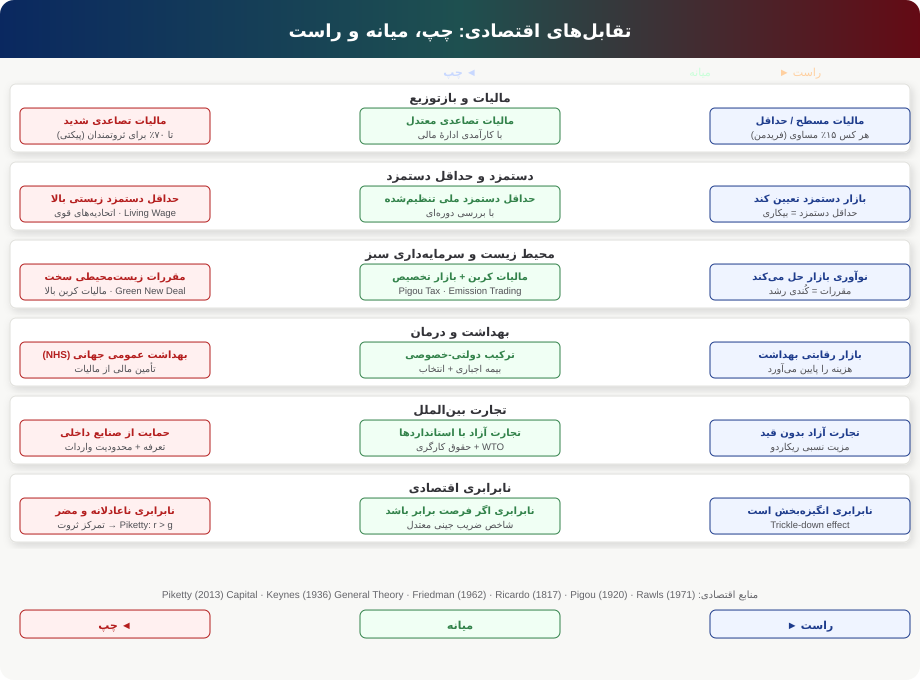
\includegraphics[width=\linewidth]{infographic-economy}
\caption{مقایسهٔ رویکردهای اقتصادی چپ، میانه و راست در شش حوزهٔ اصلی}
\label{fig:economy}
\end{figure}

\begin{historybox}[پیکتی و بازگشت نابرابری]
\person{توما پیکتی} در \book{سرمایه در قرن بیست‌ویکم} (۲۰۱۳)
با بررسی داده‌های سیصدسالهٔ ۲۰ کشور نشان داد که نرخ بازده سرمایه ($r$)
همواره از نرخ رشد اقتصادی ($g$) بیشتر است:
\[
r > g \implies \text{تمرکز ثروت افزایش می‌یابد}
$$
نتیجه: بدون مداخلهٔ دولت، نابرابری به‌صورت ساختاری افزایش می‌یابد.
پیکتی راه‌حل پیشنهادی خود را مالیات تصاعدی جهانی بر ثروت اعلام کرد.\\[4pt]
\textbf{\textcolor{RightBlue}{\rl{نقد راست:}}}
\person{مانکیو} و \person{آجموغلو} استدلال کردند که $r>g$
لزوماً به تمرکز ثروت نمی‌انجامد و عوامل نهادی نادیده گرفته شده‌اند.\\[2pt]
{\footnotesize\en{Piketty (2013), \textit{Capital in the Twenty-First Century},
	Harvard UP.\\
	Mankiw (2015). Yes, r > g. So What? \textit{AER}, 105(5).}}
\end{historybox}

\vspace{6pt}

% ─────────────────────────────────────────────────────────────────────────────
\section*{۱۰. توسعهٔ سیاسی و اجتماعی}
% ─────────────────────────────────────────────────────────────────────────────

\begin{center}
\begin{tikzpicture}[
every node/.style={font=\small},
topic/.style={
	rectangle, rounded corners=4pt,
	fill=DarkGray!12, draw=DarkGray,
	text width=2.8cm, align=center,
	inner sep=6pt, minimum height=1cm
},
left/.style={
	rectangle, rounded corners=3pt,
	fill=LeftRed!10, draw=LeftRed,
	text width=3.4cm, align=right,
	inner sep=5pt
},
center/.style={
	rectangle, rounded corners=3pt,
	fill=CenterGreen!10, draw=CenterGreen,
	text width=3.4cm, align=center,
	inner sep=5pt
},
right/.style={
	rectangle, rounded corners=3pt,
	fill=RightBlue!10, draw=RightBlue,
	text width=3.4cm, align=left,
	inner sep=5pt
}
]

% Header row
\node[topic, fill=LeftRed!30, draw=LeftRed,
text width=3.4cm] at (-5.5, 9)
{\textbf{\textcolor{LeftRed}{\rl{چپ}}}};
\node[topic, fill=CenterGreen!30, draw=CenterGreen,
text width=3.4cm] at (0, 9)
{\textbf{\textcolor{CenterGreen}{\rl{میانه}}}};
\node[topic, fill=RightBlue!30, draw=RightBlue,
text width=3.4cm] at (5.5, 9)
{\textbf{\textcolor{RightBlue}{\rl{راست}}}};

% ── Row 1: آموزش ──
\node[topic] at (0,7.5) {\rl{آموزش}};
\node[left]  at (-5.5,7.5) {
	\rl{آموزش رایگان و عمومی}\\
	\rl{برابری دسترسی}\\
	{\footnotesize\en{Dewey, Freire}}
};
\node[center] at (0,7.5) {
	\rl{آموزش عمومی باکیفیت}\\
	\rl{+ گزینهٔ خصوصی}
};
\node[right] at (5.5,7.5) {
	\rl{رقابت مدارس}\\
	\rl{کوپن آموزشی}\\
	{\footnotesize\en{Friedman (1955)}}
};

% Separator line
\draw[DarkGray!30, line width=0.4pt] (-7.5,6.75) -- (7.5,6.75);

% ── Row 2: سیاست جنسیتی ──
\node[topic] at (0,6.1) {\rl{جنسیت و هویت}};
\node[left]  at (-5.5,6.1) {
	\rl{حقوق اقلیت‌های جنسی}\\
	\rl{سهمیهٔ جنسیتی}\\
	{\footnotesize\en{Butler, Fraser}}
};
\node[center] at (0,6.1) {
	\rl{برابری قانونی}\\
	\rl{بدون تبعیض}
};
\node[right] at (5.5,6.1) {
	\rl{نقش‌های سنتی}\\
	\rl{خانواده محور}\\
	{\footnotesize\en{Burke, Scruton}}
};

\draw[DarkGray!30, line width=0.4pt] (-7.5,5.35) -- (7.5,5.35);

% ── Row 3: مهاجرت ──
\node[topic] at (0,4.65) {\rl{مهاجرت}};
\node[left]  at (-5.5,4.65) {
	\rl{مرزهای باز}\\
	\rl{حمایت از پناهندگان}\\
	{\footnotesize\en{Carens (1987)}}
};
\node[center] at (0,4.65) {
	\rl{مهاجرت تنظیم‌شده}\\
	\rl{ادغام فرهنگی}
};
\node[right] at (5.5,4.65) {
	\rl{مهاجرت کنترل‌شده}\\
	\rl{اولویت شهروندان}\\
	{\footnotesize\en{Walzer (1983)}}
};

\draw[DarkGray!30, line width=0.4pt] (-7.5,3.9) -- (7.5,3.9);

% ── Row 4: جرم و کیفر ──
\node[topic] at (0,3.2) {\rl{جرم و مجازات}};
\node[left]  at (-5.5,3.2) {
	\rl{علت اجتماعی جرم}\\
	\rl{اصلاح، نه تنبیه}\\
	{\footnotesize\en{Foucault (1975)}}
};
\node[center] at (0,3.2) {
	\rl{توانبخشی + بازدارندگی}\\
	\rl{عدالت ترمیمی}
};
\node[right] at (5.5,3.2) {
	\rl{مسئولیت فردی}\\
	\rl{مجازات بازدارنده}\\
	{\footnotesize\en{Wilson \& Herrnstein}}
};

\draw[DarkGray!30, line width=0.4pt] (-7.5,2.45) -- (7.5,2.45);

% ── Row 5: محیط زیست ──
\node[topic] at (0,1.75) {\rl{محیط زیست}};
\node[left]  at (-5.5,1.75) {
	\rl{انقلاب سبز ساختاری}\\
	\rl{Green New Deal}\\
	{\footnotesize\en{Klein (2014)}}
};
\node[center] at (0,1.75) {
	\rl{مالیات کربن}\\
	\rl{توسعهٔ پایدار}\\
	{\footnotesize\en{Pigou (1920)}}
};
\node[right] at (5.5,1.75) {
	\rl{نوآوری بازار}\\
	\rl{محیط‌زیست خصوصی}\\
	{\footnotesize\en{Anderson \& Leal}}
};

\draw[DarkGray!30, line width=0.4pt] (-7.5,1.0) -- (7.5,1.0);

% ── Row 6: دین و سیاست ──
\node[topic] at (0,0.3) {\rl{دین و دولت}};
\node[left]  at (-5.5,0.3) {
	\rl{جدایی کامل}\\
	\rl{لائیسیته}\\
	{\footnotesize\en{Mill (1859)}}
};
\node[center] at (0,0.3) {
	\rl{سکولاریسم ملایم}\\
	\rl{آزادی دینی همگان}
};
\node[right] at (5.5,0.3) {
	\rl{دین پایهٔ نظم اجتماعی}\\
	\rl{ارزش‌های سنتی}\\
	{\footnotesize\en{Burke, Scruton}}
};

\end{tikzpicture}
\end{center}

\vspace{6pt}

% ─────────────────────────────────────────────────────────────────────────────
\section*{۱۱. رقابت در برابر همکاری}
% ─────────────────────────────────────────────────────────────────────────────

\begin{center}
\begin{tikzpicture}[scale=0.95, every node/.style={font=\small}]

% Competition box
\node[draw=RightBlue, fill=RightBlue!8,
rounded corners=6pt,
minimum width=6.2cm, minimum height=7cm,
align=center] (comp) at (2.5,3) {};
\node[font=\bfseries\large, color=RightBlue] at (2.5,6.2)
{\rl{رقابت}};
\node[font=\footnotesize, color=RightBlue] at (2.5,5.7)
{\en{Competition}};

% Competition arguments
\node[align=right, text width=5.5cm] at (2.5,4.2) {
	\rl{• نوآوری: شرکت‌های رقیب نوآوری می‌کنند (شومپتر)}\\
	\rl{• کارایی: قیمت‌ها اطلاعات منتقل می‌کنند (هایک)}\\
	\rl{• انتخاب: مصرف‌کننده قدرت دارد}\\
	\rl{• انگیزه: پاداش استعداد و تلاش}
};

% Critique of competition
\node[draw=LeftRed!50, fill=LeftRed!6,
rounded corners=3pt,
align=right, text width=5.4cm,
inner sep=6pt] at (2.5,1.4) {
	\textbf{\textcolor{LeftRed}{\rl{نقدها:}}}\\
	\rl{• انحصار طبیعی (مارکس)}\\
	\rl{• استثمار ضعیف توسط قوی}\\
	\rl{• شکست بازار در کالاهای عمومی}\\
	{\footnotesize\en{Stiglitz (2012),
			\textit{The Price of Inequality}}}
};

% Cooperation box
\node[draw=LeftRed, fill=LeftRed!8,
rounded corners=6pt,
minimum width=6.2cm, minimum height=7cm,
align=center] (coop) at (11.5,3) {};
\node[font=\bfseries\large, color=LeftRed] at (11.5,6.2)
{\rl{همکاری}};
\node[font=\footnotesize, color=LeftRed] at (11.5,5.7)
{\en{Cooperation}};

% Cooperation arguments
\node[align=right, text width=5.5cm] at (11.5,4.2) {
	\rl{• همبستگی اجتماعی (دورکیم)}\\
	\rl{• کاهش نابرابری و تنش}\\
	\rl{• کالاهای عمومی بهتر تأمین می‌شوند}\\
	\rl{• اعتماد اجتماعی = سرمایه اجتماعی}
};

% Critique of cooperation
\node[draw=RightBlue!50, fill=RightBlue!6,
rounded corners=3pt,
align=right, text width=5.4cm,
inner sep=6pt] at (11.5,1.4) {
	\textbf{\textcolor{RightBlue}{\rl{نقدها:}}}\\
	\rl{• مشکل سوارکار آزاد (Olson)}\\
	\rl{• بوروکراسی و ناکارآمدی}\\
	\rl{• کاهش انگیزهٔ فردی}\\
	{\footnotesize\en{Olson (1965),
			\textit{The Logic of Collective Action}}}
};

% Middle - synthesis
\node[draw=CenterGreen, fill=CenterGreen!10,
rounded corners=6pt,
minimum width=3.8cm, minimum height=3cm,
align=center, inner sep=8pt] at (7,3.5) {
	\textbf{\textcolor{CenterGreen}{\rl{ترکیب}}}\\[4pt]
	\rl{رقابت تنظیم‌شده}\\
	\rl{بازار + شبکه ایمنی}\\
	\rl{اتحادیه + شرکت}\\[4pt]
	{\footnotesize\en{Ostrom (1990)\\
			\textit{Governing the Commons}}}
};

% Arrows
\draw[<->, CenterGreen, line width=2pt]
(comp.east) -- (coop.west)
node[midway, above, font=\bfseries, color=CenterGreen]
{\rl{تعادل پویا}};

\draw[->, CenterGreen!60, line width=1.2pt, dashed]
(7,2) -- (4,1.5);
\draw[->, CenterGreen!60, line width=1.2pt, dashed]
(7,2) -- (10,1.5);

\end{tikzpicture}
\end{center}

\vspace{4pt}

\begin{personbox}[الینور استروم: فراتر از دوگانهٔ دولت–بازار]
\person{الینور استروم}، برندهٔ جایزهٔ نوبل اقتصاد ۲۰۰۹، در
\book{حکمرانی منابع مشترک} نشان داد که جوامع می‌توانند
بدون دولت و بدون بازار، از طریق «نهادهای خودسامان» منابع مشترک
را به‌شکل پایدار مدیریت کنند.
این یافته هر دو دیدگاه ساده‌انگارانهٔ «دولت‌گرایی محض» و «بازارگرایی محض»
را به چالش می‌کشد.\\[4pt]
{\footnotesize\en{Ostrom, E. (1990). \textit{Governing the Commons:
		The Evolution of Institutions for Collective Action}. Cambridge UP.}}
\end{personbox}

\ornamentalrule

% ─────────────────────────────────────────────────────────────────────────────
\section*{۱۲. نظم در برابر آزادی}
% ─────────────────────────────────────────────────────────────────────────────

\begin{center}
\begin{tikzpicture}[scale=0.95, every node/.style={font=\small}]

% Main spectrum
\shade[left color=DarkGray!80, right color=CenterGreen!70,
shading angle=0]
(0,-0.25) rectangle (14,0.25);
\draw[DarkGray, line width=1pt] (0,-0.25) rectangle (14,0.25);

% Pole labels
\node[above, font=\bfseries, color=DarkGray] at (0.5,0.3)
{\rl{نظم مطلق}};
\node[above, font=\bfseries, color=CenterGreen] at (13.5,0.3)
{\rl{آزادی مطلق}};

% Positions
\foreach \x/\col/\lbl/\sub in {
	1/DarkGray!80/{توتالیتاریسم}/{هیتلر، استالین}،
	3.5/RightBlueDark/{اقتدارگرایی}/{پینوشه، فرانکو}،
	6/RightBlue/{محافظه‌کاری}/{برک، اوکشات}،
	8.5/CenterGreen/{دموکراسی لیبرال}/{لاک، میل}،
	11/GoldDark/{لیبرتارینیسم}/{نوزیک، رُتبارد}،
	13/PurpleAccent/{آنارشیسم}/{باکونین، کروپوتکین}%
}{
	\fill[\col] (\x,0) circle (5.5pt);
	\node[below, align=center, text width=2.2cm] at (\x,-0.4)
	{\textcolor{\col}{\rl{\lbl}}\\
		{\tiny\textcolor{MediumGray}{\rl{\sub}}}};
}

% Optimal zone bracket
\draw[CenterGreen, line width=1.5pt,
decorate, decoration={brace, amplitude=8pt, mirror}]
(6.5,-1.6) -- (10,-1.6);
\node[below, color=CenterGreen, font=\bfseries] at (8.25,-1.9)
{\rl{محدودهٔ دموکراسی‌های پایدار}};

% Hobbes-Locke tension
\draw[<->, OrangeAccent, line width=1pt, dashed]
(1,1) -- (8.5,1)
node[midway, above, font=\footnotesize, color=OrangeAccent]
{\rl{هابز: نظم ← ← ← → → → لاک: آزادی}};

\end{tikzpicture}
\end{center}

\begin{quotebox}[هابز در برابر لاک]
\begin{tcolorbox}[
enhanced, colback=white, colframe=white,
sidebyside, sidebyside align=top,
lefthand width=0.47\textwidth,
boxrule=0pt
]
\begin{tcolorbox}[
	colback=DarkGray!8, colframe=DarkGray,
	boxrule=1pt, arc=4pt,
	title={\rl{هابز: لویاتان}},
	fonttitle=\bfseries, coltitle=white,
	attach boxed title to top right={yshift=-2mm,xshift=-4mm},
	boxed title style={colback=DarkGray, rounded corners}
	]
	\textit{«انسان در حالت طبیعی گرگ انسان است.
		بدون دولت قدرتمند، زندگی تنها، فقیرانه،
		کثیف، وحشیانه و کوتاه است.»}\\[4pt]
	← نظم مقدم بر آزادی\\
	← قرارداد اجتماعی = تسلیم قدرت\\
	{\footnotesize\en{Hobbes (1651), \textit{Leviathan}}}
\end{tcolorbox}
\tcblower
\begin{tcolorbox}[
	colback=CenterGreen!8, colframe=CenterGreen,
	boxrule=1pt, arc=4pt,
	title={\rl{لاک: حکومت مشروط}},
	fonttitle=\bfseries, coltitle=white,
	attach boxed title to top right={yshift=-2mm,xshift=-4mm},
	boxed title style={colback=CenterGreen, rounded corners}
	]
	\textit{«قدرت سیاسی از رضایت اداره‌شوندگان
		سرچشمه می‌گیرد. حکومتی که حقوق طبیعی را
		نقض کند مشروعیت خود را از دست می‌دهد.»}\\[4pt]
	← آزادی حق طبیعی است\\
	← قرارداد اجتماعی = محدودیت دولت\\
	{\footnotesize\en{Locke (1689), \textit{Two Treatises of Government}}}
\end{tcolorbox}
\end{tcolorbox}
\end{quotebox}

\ornamentalrule

% ─────────────────────────────────────────────────────────────────────────────
\section*{۱۳. جدول جامع تقابل‌ها}
% ─────────────────────────────────────────────────────────────────────────────

\begin{longtable}{
>{\columncolor{DarkGray!8}}r
p{3.8cm}
p{3.8cm}
p{3.2cm}
p{3cm}
}

\rowcolor{DarkGray!25}
\textbf{حوزه / تقابل} &
\textbf{\textcolor{LeftRed}{قطب چپ}} &
\textbf{\textcolor{CenterGreen}{میانه}} &
\textbf{\textcolor{RightBlue}{قطب راست}} &
\textbf{منبع کلیدی}
\\\hline
\endfirsthead

\rowcolor{DarkGray!15}
\multicolumn{5}{r}{\footnotesize\rl{ادامهٔ جدول تقابل‌ها}}\\
\rowcolor{DarkGray!25}
\textbf{حوزه / تقابل} &
\textbf{\textcolor{LeftRed}{قطب چپ}} &
\textbf{\textcolor{CenterGreen}{میانه}} &
\textbf{\textcolor{RightBlue}{قطب راست}} &
\textbf{منبع کلیدی}
\\\hline
\endhead

\hline
\multicolumn{5}{l}{\footnotesize\rl{ادامه دارد...}}
\endfoot

\hline
\endlastfoot

% ── اقتصاد ──
\rowcolor{RightBlue!6}
\multicolumn{5}{r}{
\textbf{\textcolor{RightBlue}{\rl{▸ حوزهٔ اقتصادی}}}}
\\\hline

مالکیت &
مالکیت اجتماعی و عمومی &
اقتصاد مختلط &
مالکیت خصوصی مقدس &
\en{\footnotesize Nozick (1974)}
\\\hline

مالیات &
تصاعدی شدید تا ۷۰٪ &
تصاعدی معتدل &
مسطح یا حداقلی &
\en{\footnotesize Piketty (2013)}
\\\hline

دستمزد &
حداقل دستمزد زیستی + اتحادیه &
حداقل دستمزد ملی &
بازار تعیین کند &
\en{\footnotesize Stiglitz (2012)}
\\\hline

تجارت &
حمایت از صنایع داخلی &
تجارت آزاد با استانداردها &
آزادسازی کامل &
\en{\footnotesize Ricardo (1817)}
\\\hline

بیکاری &
علت ساختاری، دولت مسئول &
ترکیبی &
انتخاب یا کم‌کاری فردی &
\en{\footnotesize Keynes (1936)}
\\\hline

نابرابری &
تهدید دموکراسی &
نابرابری معتدل قابل قبول &
انگیزه‌بخش و ضروری &
\en{\footnotesize Rawls (1971)}
\\\hline

% ── سیاسی ──
\rowcolor{LeftRed!6}
\multicolumn{5}{r}{
\textbf{\textcolor{LeftRed}{\rl{▸ حوزهٔ سیاسی}}}}
\\\hline

دموکراسی &
مشارکتی + اقتصادی &
لیبرال نمایندگی &
قانون اساسی محدود &
\en{\footnotesize Habermas (1996)}
\\\hline

نقش دولت &
هدایت‌گر و تنظیم‌گر &
تسهیل‌گر &
حداقلی: نگهبان شب &
\en{\footnotesize Hayek (1944)}
\\\hline

آزادی مدنی &
آزادی مثبت &
هر دو &
آزادی منفی &
\en{\footnotesize Berlin (1969)}
\\\hline

نظم سیاسی &
تغییر بنیادین &
اصلاح تدریجی &
حفظ سنت‌ها &
\en{\footnotesize Burke (1790)}
\\\hline

ملت‌گرایی &
انترناسیونالیسم &
همکاری + حاکمیت ملی &
ناسیونالیسم &
\en{\footnotesize Walzer (1983)}
\\\hline

حقوق اقلیت &
حمایت فعال + سهمیه‌بندی &
حمایت قانونی &
برابری در برابر قانون &
\en{\footnotesize Dworkin (2000)}
\\\hline

% ── اجتماعی ──
\rowcolor{CenterGreen!6}
\multicolumn{5}{r}{
\textbf{\textcolor{CenterGreen}{\rl{▸ حوزهٔ اجتماعی}}}}
\\\hline

آموزش &
عمومی رایگان، برابر &
عمومی باکیفیت + خصوصی &
رقابت و کوپن &
\en{\footnotesize Friedman (1955)}
\\\hline

بهداشت &
NHS: عمومی جهانی &
بیمه اجباری &
بازار رقابتی &
\en{\footnotesize Beveridge (1942)}
\\\hline

محیط زیست &
مقررات سخت + انقلاب سبز &
مالیات کربن &
نوآوری بازار &
\en{\footnotesize Pigou (1920)}
\\\hline

جرم &
علل اجتماعی + اصلاح &
توانبخشی + بازدارندگی &
مسئولیت فرد + مجازات &
\en{\footnotesize Foucault (1975)}
\\\hline

مهاجرت &
مرزهای باز، حقوق پناهنده &
مهاجرت تنظیم‌شده &
کنترل سخت مرز &
\en{\footnotesize Carens (1987)}
\\\hline

خانواده &
تکثر شکل خانواده &
حمایت از خانواده + تکثر &
خانوادهٔ سنتی &
\en{\footnotesize Scruton (2001)}
\\\hline

دین &
جدایی کامل لائیسیته &
سکولاریسم ملایم &
دین پایهٔ نظم اجتماعی &
\en{\footnotesize Mill (1859)}
\\\hline

% ── عدالت ──
\rowcolor{GoldAccent!10}
\multicolumn{5}{r}{
\textbf{\textcolor{GoldDark}{\rl{▸ حوزهٔ عدالت}}}}
\\\hline

عدالت توزیعی &
برابری نتیجه &
برابری فرصت &
استحقاق &
\en{\footnotesize Rawls vs. Nozick}
\\\hline

عدالت جبرانی &
اقدام مثبت فعال &
جبران هدفمند &
مخالف سهمیه‌بندی &
\en{\footnotesize Fraser (1997)}
\\\hline

عدالت رویه‌ای &
فرآیند + نتیجه &
رویهٔ منصفانه &
رویهٔ صحیح = نتیجهٔ عادل &
\en{\footnotesize Fuller (1964)}
\\\hline

مسئولیت &
ساختارهای اجتماعی &
فرد + ساختار &
مسئولیت فردی &
\en{\footnotesize Sandel (2009)}
\\\hline

مالیات = سرقت؟ &
مالیات = همبستگی &
مالیات = قرارداد اجتماعی &
نوزیک: مالیات اجباری نادرست &
\en{\footnotesize Nozick (1974)}
\\\hline

\caption{جدول جامع تقابل‌های موضوعی در ۲۴ حوزه با مستندات آکادمیک}
\label{tab:comprehensive}
\end{longtable}

\vspace{8pt}

% ─────────────────────────────────────────────────────────────────────────────
\section*{۱۴. کوتاه‌مدت در برابر بلندمدت}
% ─────────────────────────────────────────────────────────────────────────────

\begin{center}
\begin{tikzpicture}[every node/.style={font=\small}]

% Timeline arrow
\draw[line width=3pt, -{Stealth[length=10pt, width=8pt]},
color=DarkGray] (0,0) -- (13,0);

% Time markers
\foreach \x/\yr in {1/امروز, 3.5/{۵ سال}, 6/{۲۰ سال},
	9/{۵۰ سال}, 12/{نسل آینده}} {
	\draw[DarkGray!50, line width=0.8pt] (\x,-0.2) -- (\x,0.2);
	\node[below, font=\footnotesize, color=DarkGray!70] at (\x,-0.3)
	{\rl{\yr}};
}

% Short-term focus (right politics)
\node[draw=RightBlue, fill=RightBlue!10,
rounded corners=5pt, align=right,
text width=4.5cm, inner sep=7pt] at (2.5,2.5) {
	\textbf{\textcolor{RightBlue}{\rl{تمرکز کوتاه‌مدت (راست)}}}\\[3pt]
	\rl{• سود سه‌ماهه}\\
	\rl{• انتخابات بعدی}\\
	\rl{• نتایج فوری بازار}\\[2pt]
	{\footnotesize\en{Keynes: «در بلندمدت همه مرده‌ایم»}}
};

% Arrow from box to timeline
\draw[->, RightBlue!50, line width=1pt, dashed]
(2.5,1.4) -- (2.5,0.3);

% Long-term focus (left/green politics)
\node[draw=CenterGreen, fill=CenterGreen!10,
rounded corners=5pt, align=right,
text width=4.5cm, inner sep=7pt] at (10,2.5) {
	\textbf{\textcolor{CenterGreen}{\rl{تمرکز بلندمدت (چپ / سبز)}}}\\[3pt]
	\rl{• تغییر اقلیم}\\
	\rl{• نابرابری بین‌نسلی}\\
	\rl{• توسعهٔ پایدار}\\[2pt]
	{\footnotesize\en{Rawls: عدالت بین‌نسلی}}
};

\draw[->, CenterGreen!50, line width=1pt, dashed]
(10,1.4) -- (10,0.3);

% Tension marker
\draw[<->, OrangeAccent, line width=1.5pt]
(4.5,2.5) -- (8,2.5)
node[midway, above, color=OrangeAccent, font=\bfseries]
{\rl{تنش اصلی}};

% Specific issues
\node[align=center, font=\footnotesize,
color=RightBlue] at (2.5,-1.2) {
	\rl{کاهش مالیات امروز}\\
	\rl{بدهی = مشکل نسل بعد}
};

\node[align=center, font=\footnotesize,
color=CenterGreen] at (10,-1.2) {
	\rl{سرمایه‌گذاری در آموزش}\\
	\rl{مالیات کربن}
};

\end{tikzpicture}
\end{center}

\vspace{8pt}

% ─────────────────────────────────────────────────────────────────────────────
\section*{۱۵. منابع آکادمیک دست‌اول}
% ─────────────────────────────────────────────────────────────────────────────

\begin{summarybox}

\begin{center}
\textbf{\large\rl{کتابخانهٔ پایه: آثار دست‌اول}}
\end{center}

\mediumspace

\begin{tikzpicture}[every node/.style={font=\footnotesize}]

% Three columns: Left, Center, Right
% Left column header
\node[draw=LeftRed, fill=LeftRed!15,
rounded corners=4pt,
text width=4.2cm, align=center,
inner sep=6pt] at (0,12) {
	\textbf{\textcolor{LeftRed}{\rl{منابع چپ}}}
};

% Left books
\foreach \y/\auth/\ttl/\yr in {
	10.8/{Marx \& Engels}/{The Communist Manifesto}/{1848},
	9.6/{Marx, K.}/{Das Kapital, Vol. 1}/{1867},
	8.4/{Rousseau, J.J.}/{The Social Contract}/{1762},
	7.2/{Rawls, J.}/{A Theory of Justice}/{1971},
	6.0/{Piketty, T.}/{Capital in the 21st Century}/{2013},
	4.8/{Fraser, N.}/{Justice Interruptus}/{1997},
	3.6/{Young, I.M.}/{Justice and Difference}/{1990},
	2.4/{Freire, P.}/{Pedagogy of the Oppressed}/{1968},
	1.2/{Habermas, J.}/{Between Facts and Norms}/{1996}%
}{
	\node[draw=LeftRed!30, fill=LeftRed!4,
	rounded corners=2pt,
	text width=4.2cm, align=right,
	inner sep=4pt] at (0,\y) {
		\textbf{\en{\auth}}\\
		\textit{\en{\ttl}}\\
		\textcolor{MediumGray}{\en{\yr}}
	};
}

% Center column header
\node[draw=CenterGreen, fill=CenterGreen!15,
rounded corners=4pt,
text width=4.2cm, align=center,
inner sep=6pt] at (5,12) {
	\textbf{\textcolor{CenterGreen}{\rl{منابع میانه}}}
};

\foreach \y/\auth/\ttl/\yr in {
	10.8/{Rawls, J.}/{Political Liberalism}/{1993},
	9.6/{Sandel, M.}/{Justice: What's Right?}/{2009},
	8.4/{Dworkin, R.}/{Sovereign Virtue}/{2000},
	7.2/{Keynes, J.M.}/{General Theory}/{1936},
	6.0/{Giddens, A.}/{The Third Way}/{1998},
	4.8/{Dahl, R.}/{Democracy and Its Critics}/{1989},
	3.6/{Sen, A.}/{Development as Freedom}/{1999},
	2.4/{Ostrom, E.}/{Governing the Commons}/{1990},
	1.2/{Mill, J.S.}/{On Liberty}/{1859}%
}{
	\node[draw=CenterGreen!30, fill=CenterGreen!4,
	rounded corners=2pt,
	text width=4.2cm, align=right,
	inner sep=4pt] at (5,\y) {
		\textbf{\en{\auth}}\\
		\textit{\en{\ttl}}\\
		\textcolor{MediumGray}{\en{\yr}}
	};
}

% Right column header
\node[draw=RightBlue, fill=RightBlue!15,
rounded corners=4pt,
text width=4.2cm, align=center,
inner sep=6pt] at (10,12) {
	\textbf{\textcolor{RightBlue}{\rl{منابع راست}}}
};

\foreach \y/\auth/\ttl/\yr in {
	10.8/{Hayek, F.A.}/{The Road to Serfdom}/{1944},
	9.6/{Hayek, F.A.}/{The Constitution of Liberty}/{1960},
	8.4/{Nozick, R.}/{Anarchy, State \& Utopia}/{1974},
	7.2/{Friedman, M.}/{Capitalism and Freedom}/{1962},
	6.0/{Burke, E.}/{Reflections on Revolution}/{1790},
	4.8/{Locke, J.}/{Two Treatises of Government}/{1689},
	3.6/{Hobbes, T.}/{Leviathan}/{1651},
	2.4/{Sowell, T.}/{A Conflict of Visions}/{1987},
	1.2/{Scruton, R.}/{The Meaning of Conservatism}/{1980}%
}{
	\node[draw=RightBlue!30, fill=RightBlue!4,
	rounded corners=2pt,
	text width=4.2cm, align=right,
	inner sep=4pt] at (10,\y) {
		\textbf{\en{\auth}}\\
		\textit{\en{\ttl}}\\
		\textcolor{MediumGray}{\en{\yr}}
	};
}

\end{tikzpicture}

\end{summarybox}

\vspace{8pt}

\begin{questionbox}
\begin{enumerate}[leftmargin=*, itemsep=8pt]
\item اگر «پشت پردهٔ جهل» رولز قرار داشتید،
کدام نظام توزیع ثروت را انتخاب می‌کردید و چرا؟

\item آیا دموکراسی مشارکتی چپ و دموکراسی قانون اساسی راست
می‌توانند با یکدیگر ترکیب شوند؟
چه نمونه‌های تاریخی می‌شناسید؟

\item پیکتی نشان داد $r > g$؛ آیا این به معنای
ناپایداری ذاتی سرمایه‌داری است؟
هایک چه پاسخی می‌داد؟

\item مرز میان «آزادی منفی» و «آزادی مثبت» کجاست؟
آیا حق بهداشت «آزادی مثبت» است یا حقی بنیادین‌تر؟

\item استروم نشان داد جوامع بدون دولت و بازار می‌توانند
منابع مشترک را مدیریت کنند.
این یافته چه چالشی برای هر دو طیف چپ و راست ایجاد می‌کند؟
\end{enumerate}
\end{questionbox}

\chapter*{ضمیمهٔ ۸: تقابل‌های موضوعی}
\addcontentsline{toc}{chapter}{ضمیمهٔ ۸: تقابل‌های موضوعی}
\thispagestyle{plain}

\begin{center}
  \begin{tikzpicture}
    \node[
      draw=GoldAccent, line width=1.2pt,
      fill=GoldAccent!6,
      rounded corners=6pt,
      inner sep=10pt,
      text width=0.82\linewidth,
      align=center
    ] {
      \textcolor{DarkGray}{\large\itshape
        تصویرسازی بصری از تنش‌های بنیادین اندیشهٔ سیاسی}\$$4pt]
      \textcolor{MediumGray}{\small
        هر بخش با منابع آکادمیک دست‌اول مستند شده است}
    };
  \end{tikzpicture}
\end{center}

% FIXED: ornamentalrule بدون \leaders — در این موقعیت امن است
\ornamentalrule
\vspace{6pt}

% ─────────────────────────────────────────────────────────────────
\section*{۱. طیف سیاسی: اینفوگرافیک}
% ─────────────────────────────────────────────────────────────────

\begin{figure}[H]
  \centering
  % FIXED: از PDF استفاده کنید (SVG را با Inkscape تبدیل کنید)
  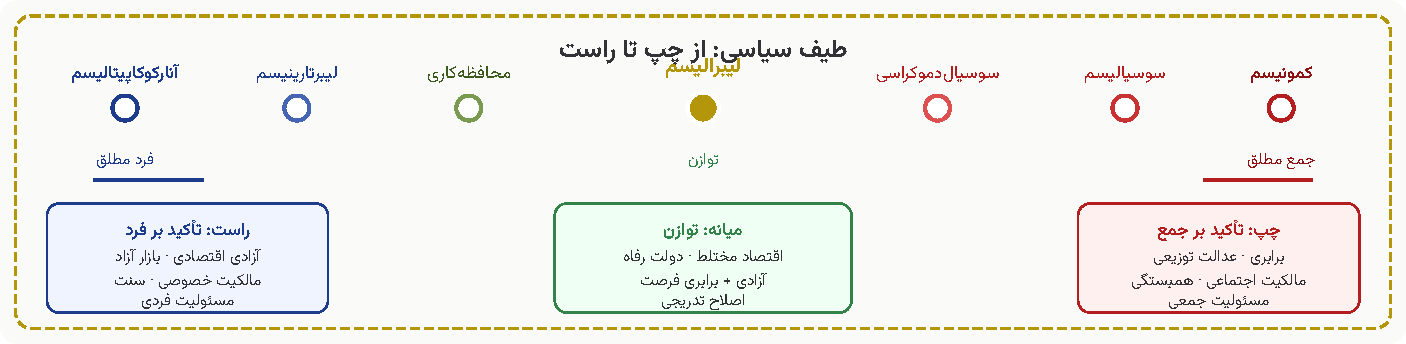
\includegraphics[width=\linewidth]{figures/infographic-spectrum.pdf}
  \caption{طیف سیاسی از آنارکو‌کاپیتالیسم تا کمونیسم}
  \label{fig:spectrum}
\end{figure}

% FIXED: rounded corners بدون مقدار
\begin{defbox}[چارچوب نظری: طیف یک‌بُعدی و محدودیت‌های آن]
تقسیم‌بندی چپ–راست از انقلاب فرانسه (۱۷۸۹) سرچشمه می‌گیرد.
\person{نولان} (۱۹۷۱) با نمودار دوبُعدی خود نشان داد این طیف خطی،
آزادی‌های شخصی را نادیده می‌گیرد.\\[4pt]
{\small\en{Bobbio, N. (1996).
\textit{Left and Right: The Significance of a Political Distinction}.
University of Chicago Press.}}
\end{defbox}

\vspace{6pt}
\ornamentalrule
\vspace{4pt}

% ─────────────────────────────────────────────────────────────────
\section*{۲. نقشهٔ دوبُعدی ایدئولوژی‌ها}
% ─────────────────────────────────────────────────────────────────

\begin{figure}[H]
  \centering
  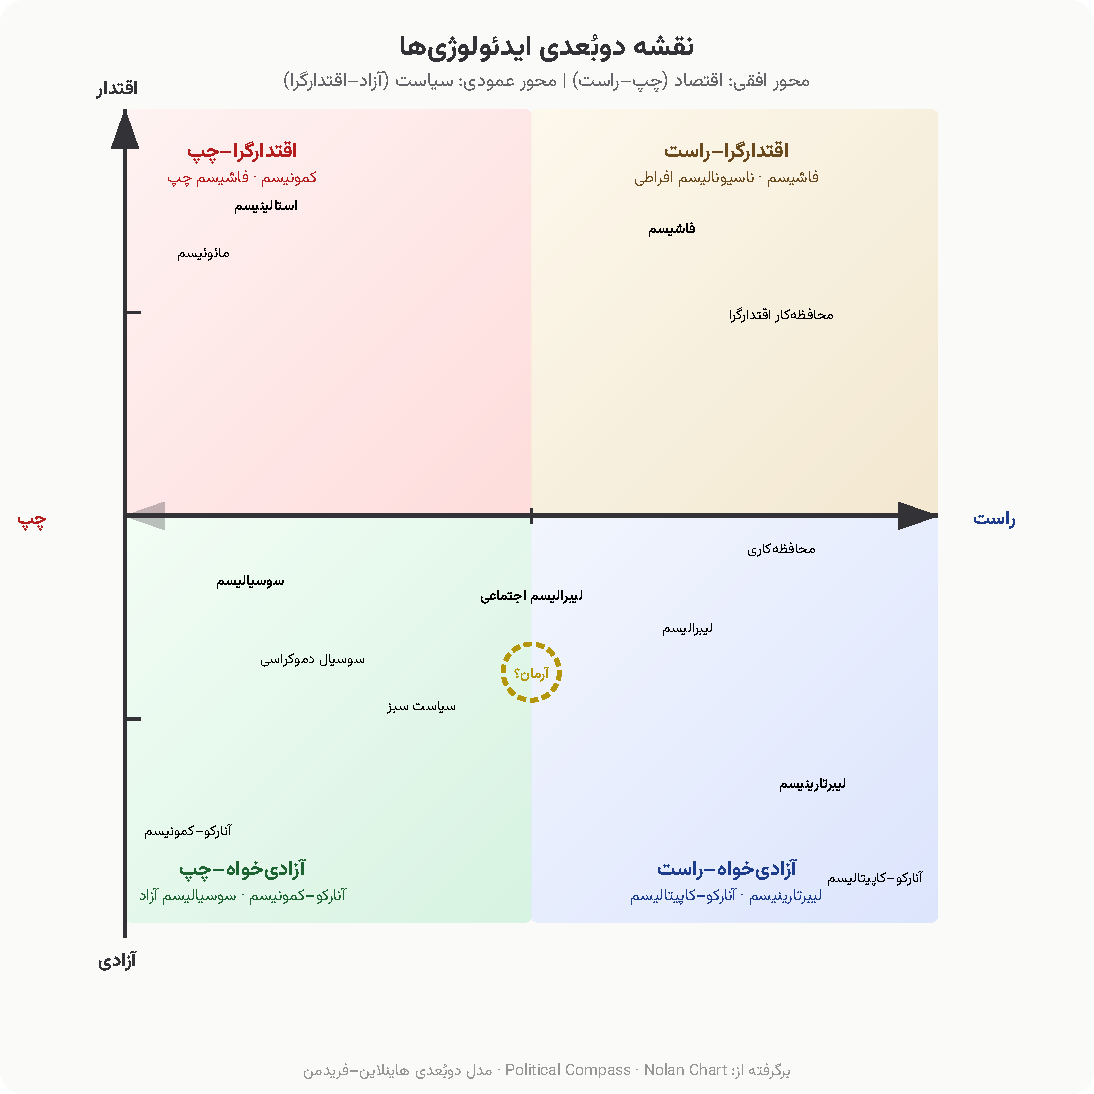
\includegraphics[width=0.92\linewidth]{figures/infographic-2axis.pdf}
  \caption{جایابی ایدئولوژی‌ها در دو محور اقتصادی و سیاسی}
  \label{fig:twoaxis}
\end{figure}

\begin{comparebox}[نمودار نولان و قطب‌نمای سیاسی]
\begin{itemize}[leftmargin=*, itemsep=3pt]
  \item \keyword{محور افقی}: اقتصاد — از مداخلهٔ کامل دولت (چپ)
        تا بازار کاملاً آزاد (راست)
  \item \keyword{محور عمودی}: سیاست — از آزادی‌های مدنی کامل (پایین)
        تا کنترل کامل دولت (بالا)
  \item \leftkw{چپ–اقتدارگرا}: استالینیسم، مائوئیسم
  \item \rightkw{راست–اقتدارگرا}: فاشیسم، ناسیونالیسم افراطی
  \item \centerkw{چپ–آزادی‌خواه}: آنارکو–کمونیسم، سوسیالیسم آزاد
  \item \rightkw{راست–آزادی‌خواه}: لیبرتارینیسم، آنارکو–کاپیتالیسم
\end{itemize}
\mediumspace
{\small\en{Nolan, D. (1971). Classifying and Analyzing
Politico-Economic Systems. \textit{The Individualist}.}}
\end{comparebox}

\ornamentalrule
\vspace{4pt}

% ─────────────────────────────────────────────────────────────────
\section*{۳. فرد در برابر جمع}
% ─────────────────────────────────────────────────────────────────

\begin{center}
\begin{tikzpicture}[scale=1, every node/.style={font=\small}]

  % گرادیان رنگی با مستطیل‌های متوالی
  \foreach \i in {0,...,27} {
    \pgfmathsetmacro{\rval}{int(30 + \i*5)}
    \pgfmathsetmacro{\bval}{int(140 - \i*5)}
    \definecolor{gradcol}{RGB}{\rval,60,\bval}
    \fill[gradcol] (\i*0.5, -0.22) rectangle (\i*0.5+0.55, 0.22);
  }
  \draw[DarkGray, line width=0.8pt] (0,-0.22) rectangle (14,0.22);

  % نقطه‌های موقعیت
  \foreach \x/\col in {
      1/RightBlueDark,
      3.2/RightBlue,
      5.5/CenterGreenDark,
      7/CenterGreen,
      9/LeftRedLight,
      11.5/LeftRed,
      13/LeftRedDark}{
    \fill[\col] (\x,0) circle (5pt);
  }

  % برچسب‌های بالا
  \node[above, align=center, text width=1.8cm]
    at (1,0.3)   {\rl{آنارکو کاپیتالیسم}};
  \node[above, align=center, text width=1.8cm]
    at (3.2,0.3) {\rl{لیبرتارینیسم}};
  \node[above, align=center, text width=1.6cm]
    at (5.5,0.3) {\rl{لیبرالیسم کلاسیک}};
  \node[above, align=center, text width=1.6cm]
    at (7,0.3)   {\rl{سوسیال دموکراسی}};
  \node[above, align=center, text width=1.6cm]
    at (9,0.3)   {\rl{سوسیالیسم دموکراتیک}};
  \node[above, align=center, text width=1.4cm]
    at (11.5,0.3){\rl{سوسیالیسم}};
  \node[above, align=center, text width=1.4cm]
    at (13,0.3)  {\rl{کمونیسم}};

  % برچسب‌های قطب
  \node[below, font=\bfseries, color=RightBlue] at (1,-0.4)
    {\rl{فرد مطلق}};
  \node[below, font=\bfseries, color=LeftRed]   at (13,-0.4)
    {\rl{جمع مطلق}};
  \node[below, font=\bfseries, color=CenterGreen] at (7,-0.4)
    {\rl{توازن}};

  % باکس‌های توضیحی
  \node[draw=RightBlue, fill=RightBlue!8, rounded corners=4pt,
        align=right, text width=4.5cm] at (1.5,4) {
    \textbf{\textcolor{RightBlue}{\rl{تأکید بر فرد:}}}\\[2pt]
    \rl{• حقوق طبیعی (لاک)}\\
    \rl{• مالکیت = شخصیت (هگل)}\\
    \rl{• مسئولیت شخصی}\\
    \rl{• رقابت انتخاب اصلح}\\[2pt]
    {\footnotesize\en{Locke (1689), Nozick (1974)}}
  };

  \node[draw=CenterGreen, fill=CenterGreen!8, rounded corners=4pt,
        align=right, text width=4cm] at (7,4) {
    \textbf{\textcolor{CenterGreen}{\rl{توازن:}}}\\[2pt]
    \rl{• رولز: پرده جهل}\\
    \rl{• سندل: جماعت‌گرایی}\\
    \rl{• حقوق + وظایف}\\[2pt]
    {\footnotesize\en{Rawls (1971)}}
  };

  \node[draw=LeftRed, fill=LeftRed!8, rounded corners=4pt,
        align=right, text width=4.5cm] at (12,4) {
    \textbf{\textcolor{LeftRed}{\rl{تأکید بر جمع:}}}\\[2pt]
    \rl{• روسو: ارادهٔ عمومی}\\
    \rl{• مارکس: آگاهی طبقاتی}\\
    \rl{• همبستگی (دورکیم)}\\
    \rl{• منافع عمومی مقدم}\\[2pt]
    {\footnotesize\en{Marx (1867), Rousseau (1762)}}
  };

  % خطوط ارتباطی
  \draw[RightBlue!40, dashed, line width=0.7pt]
    (1.5,2.3) -- (1,0.3);
  \draw[CenterGreen!40, dashed, line width=0.7pt]
    (7,2.3) -- (7,0.3);
  \draw[LeftRed!40, dashed, line width=0.7pt]
    (11.5,2.3) -- (11.5,0.3);

\end{tikzpicture}
\end{center}

\vspace{4pt}
\ornamentalrule
\vspace{4pt}

% ─────────────────────────────────────────────────────────────────
\section*{۴. آزادی منفی در برابر آزادی مثبت}
% ─────────────────────────────────────────────────────────────────

% FIXED: sidebyside tcolorbox — rounded corners بدون مقدار
\begin{tcolorbox}[
    enhanced,
    colback=VeryLightGray,
    colframe=DarkGray,
    boxrule=1.2pt,
    arc=4mm,
    sidebyside,
    sidebyside align=top,
    lefthand width=0.46\textwidth,
    drop fuzzy shadow=black!20,
    before skip=6pt, after skip=6pt
]

  \begin{center}
    \begin{tikzpicture}
      \fill[RightBlue!15, rounded corners=4pt]
           (-2.2,-0.3) rectangle (2.2,0.7);
      \node[font=\large\bfseries, color=RightBlue] at (0,0.2)
           {\rl{آزادی منفی}};
    \end{tikzpicture}\\[2pt]
    \textbf{\textcolor{RightBlue}{\rl{«آزادی از...»}}}
    \quad \en{Negative Liberty}
  \end{center}

  \begin{itemize}[leftmargin=12pt, itemsep=3pt]
    \item آزادی از دخالت دیگران
    \item آزادی از اجبار دولت
    \item حقوق منفی: حق نداشتن مزاحم
    \item «رهایم بگذارید تا زندگی کنم»
  \end{itemize}

  \mediumspace
  \textbf{\rl{نمایندگان:}}
  \person{آیزایا برلین}، \person{هایک}، \person{نوزیک}\\[3pt]
  {\small\en{Berlin, I. (1969).
  \textit{Four Concepts of Liberty}. Oxford UP.}}\\[4pt]
  \textbf{\textcolor{LeftRed}{\rl{نقد:}}}
  آزادی صوری است؛ گرسنه‌ای که آزاد است نان بدزدد
  یا گرسنگی بکشد، واقعاً آزاد است؟

\tcblower

  \begin{center}
    \begin{tikzpicture}
      \fill[LeftRed!15, rounded corners=4pt]
           (-2.2,-0.3) rectangle (2.2,0.7);
      \node[font=\large\bfseries, color=LeftRed] at (0,0.2)
           {\rl{آزادی مثبت}};
    \end{tikzpicture}\\[2pt]
    \textbf{\textcolor{LeftRed}{\rl{«آزادی برای...»}}}
    \quad \en{Positive Liberty}
  \end{center}

  \begin{itemize}[leftmargin=12pt, itemsep=3pt]
    \item آزادی برای تحقق خود
    \item توانمندسازی واقعی
    \item حقوق مثبت: حق داشتن منابع
    \item «کمکم کنید تا بتوانم»
  \end{itemize}

  \mediumspace
  \textbf{\rl{نمایندگان:}}
  \person{روسو}، \person{هگل}،
  \person{مارکس}، \person{سن}\\[3pt]
  {\small\en{Sen, A. (1999).
  \textit{Development as Freedom}. Oxford UP.}}\\[4pt]
  \textbf{\textcolor{RightBlue}{\rl{نقد:}}}
  بهانه‌ای برای پدرسالاری دولتی؛
  «آزادی» تحمیل‌شده از بالا.

\end{tcolorbox}

\vspace{4pt}

\begin{historybox}[برلین و دو مفهوم آزادی]
\person{آیزایا برلین} در سخنرانی افتتاحیهٔ استادی خود در آکسفورد (۱۹۵۸)
میان \keyword{آزادی منفی} و \keyword{آزادی مثبت} تمایز گذاشت
و هشدار داد آزادی مثبت می‌تواند به توجیه استبداد تبدیل شود.\\[3pt]
{\small\en{Berlin (1969), \textit{Four Essays on Liberty}, Oxford UP.}}
\end{historybox}

\ornamentalrule

% ─────────────────────────────────────────────────────────────────
\section*{۵. مالکیت}
% ─────────────────────────────────────────────────────────────────

\begin{figure}[H]
  \centering
  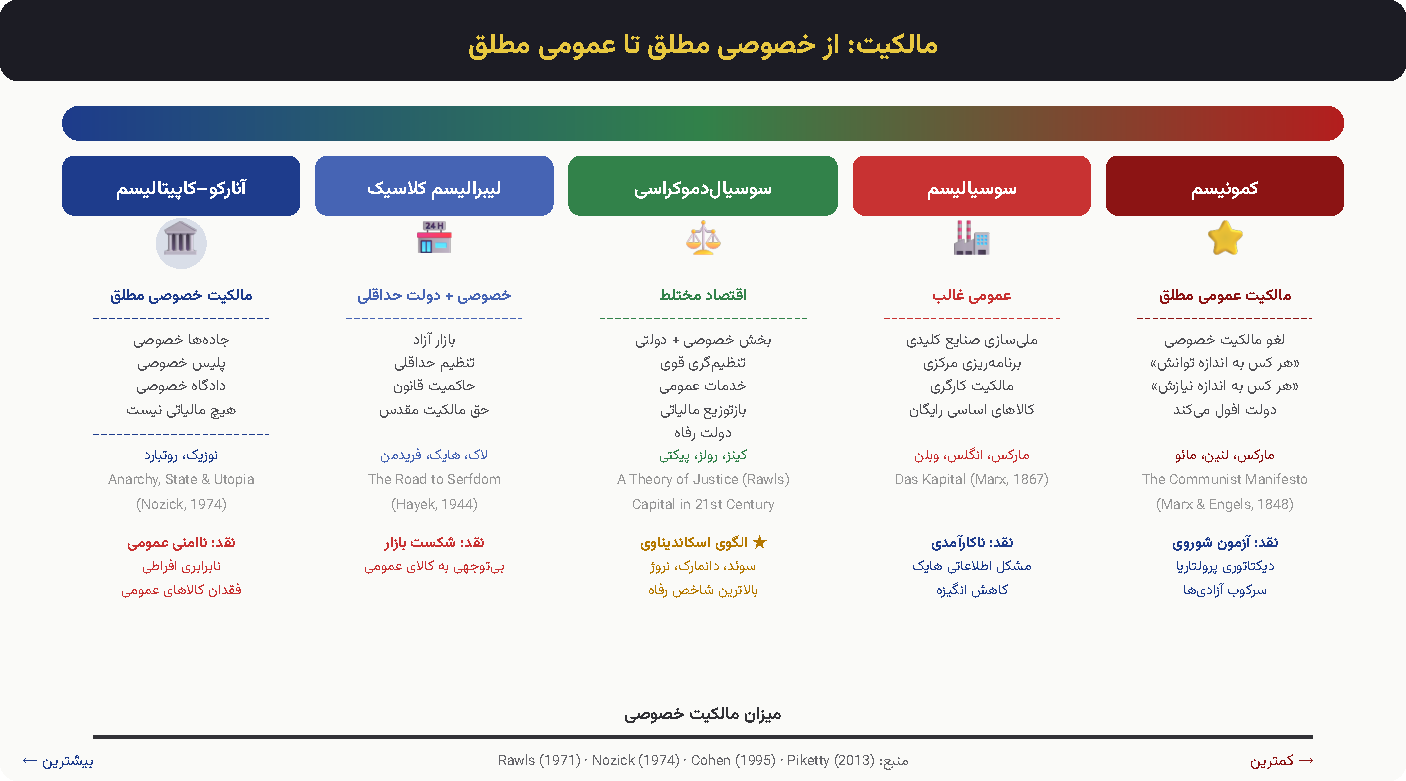
\includegraphics[width=\linewidth]{figures/infographic-property.pdf}
  \caption{طیف مالکیت از آنارکو–کاپیتالیسم تا کمونیسم}
  \label{fig:property}
\end{figure}

\begin{comparebox}[سه نظریهٔ کلاسیک مالکیت]
\begin{center}
\begin{tikzpicture}[
    node distance=0.4cm,
    box/.style={
      rectangle, rounded corners=4pt,
      minimum width=3.5cm, minimum height=2.6cm,
      align=center, text width=3.3cm,
      draw, inner sep=6pt, font=\small
    }
]
  \node[box, fill=RightBlue!10, draw=RightBlue] (locke) {
    \textbf{\textcolor{RightBlue}{\rl{لاک: کار}}}\\[3pt]
    \rl{مالکیت از کار}\\
    \rl{انسان بر کار خود حق دارد}\\[3pt]
    {\footnotesize\en{Two Treatises (1689)}}
  };
  \node[box, fill=CenterGreen!10, draw=CenterGreen,
        right=0.5cm of locke] (hegel) {
    \textbf{\textcolor{CenterGreen}{\rl{هگل: شخصیت}}}\\[3pt]
    \rl{مالکیت تجسم اراده}\\
    \rl{حقوقی بودن = مالک بودن}\\[3pt]
    {\footnotesize\en{Phil. of Right (1820)}}
  };
  \node[box, fill=LeftRed!10, draw=LeftRed,
        right=0.5cm of hegel] (marx) {
    \textbf{\textcolor{LeftRed}{\rl{مارکس: استثمار}}}\\[3pt]
    \rl{مالکیت ابزار سلطه}\\
    \rl{ارزش اضافی از کارگر}\\[3pt]
    {\footnotesize\en{Das Kapital (1867)}}
  };
  \node[box, fill=GoldAccent!10, draw=GoldAccent,
        right=0.5cm of marx] (nozick) {
    \textbf{\textcolor{GoldDark}{\rl{نوزیک: استحقاق}}}\\[3pt]
    \rl{مالکیت اکتسابی عادلانه}\\
    \rl{انتقال داوطلبانه}\\[3pt]
    {\footnotesize\en{Anarchy, State (1974)}}
  };
\end{tikzpicture}
\end{center}
\end{comparebox}

\ornamentalrule

% ─────────────────────────────────────────────────────────────────
\section*{۶. رویکرد به دموکراسی}
% ─────────────────────────────────────────────────────────────────

\begin{figure}[H]
  \centering
  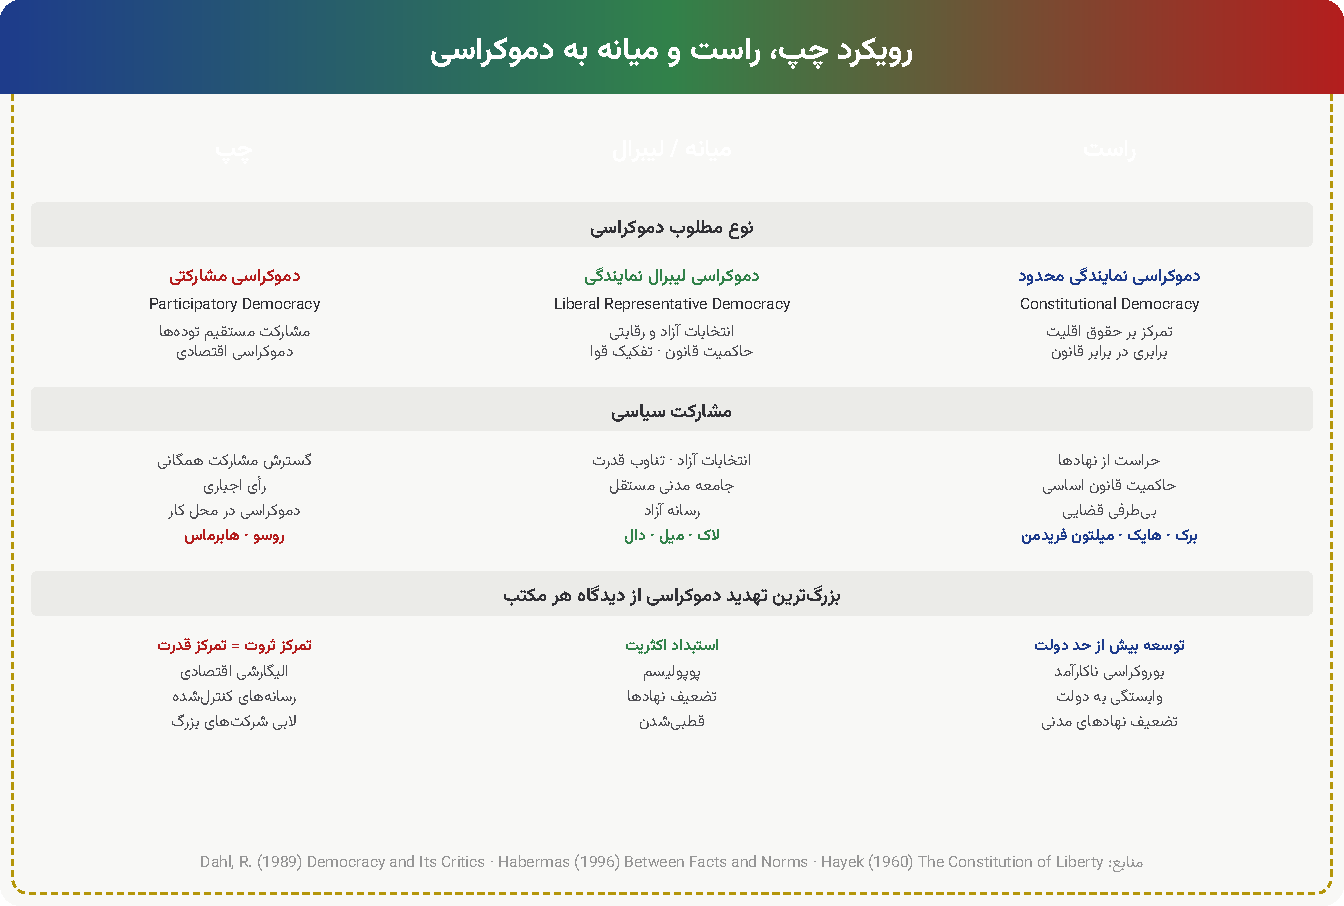
\includegraphics[width=\linewidth]{figures/infographic-democracy.pdf}
  \caption{رویکرد چپ، میانه و راست به مفهوم و انواع دموکراسی}
  \label{fig:democracy}
\end{figure}

\begin{defbox}[انواع دموکراسی و ترجیحات هر مکتب]
\begin{itemize}[leftmargin=*, itemsep=5pt]

  \item \leftkw{چپ — دموکراسی مشارکتی:}
  بر مشارکت مستقیم شهروندان تأکید دارد.
  \person{روسو} (ارادهٔ عمومی) و \person{هابرماس}
  (دموکراسی گفتگویی) از پیشگامان‌اند.\\
  {\small\en{Habermas (1996),
  \textit{Between Facts and Norms}.}}

  \item \centerkw{میانه — دموکراسی لیبرال نمایندگی:}
  \person{دال}، \person{شومپتر} و \person{لاک} پایه‌گذاران این سنت‌اند.
  \person{شومپتر} دموکراسی را «رقابت نخبگان برای کسب آرای مردم» تعریف کرد.\\
  {\small\en{Schumpeter (1942),
  \textit{Capitalism, Socialism and Democracy}.}}

  \item \rightkw{راست — دموکراسی قانون اساسی محدود:}
  \person{هایک}، \person{برک} و \person{مدیسون} بر خطر
  «استبداد اکثریت» هشدار دادند.\\
  {\small\en{Hayek (1960), \textit{The Constitution of Liberty}.}}

\end{itemize}
\end{defbox}

\ornamentalrule

% ─────────────────────────────────────────────────────────────────
\section*{۷. عدالت جبرانی}
% ─────────────────────────────────────────────────────────────────

\begin{figure}[H]
  \centering
  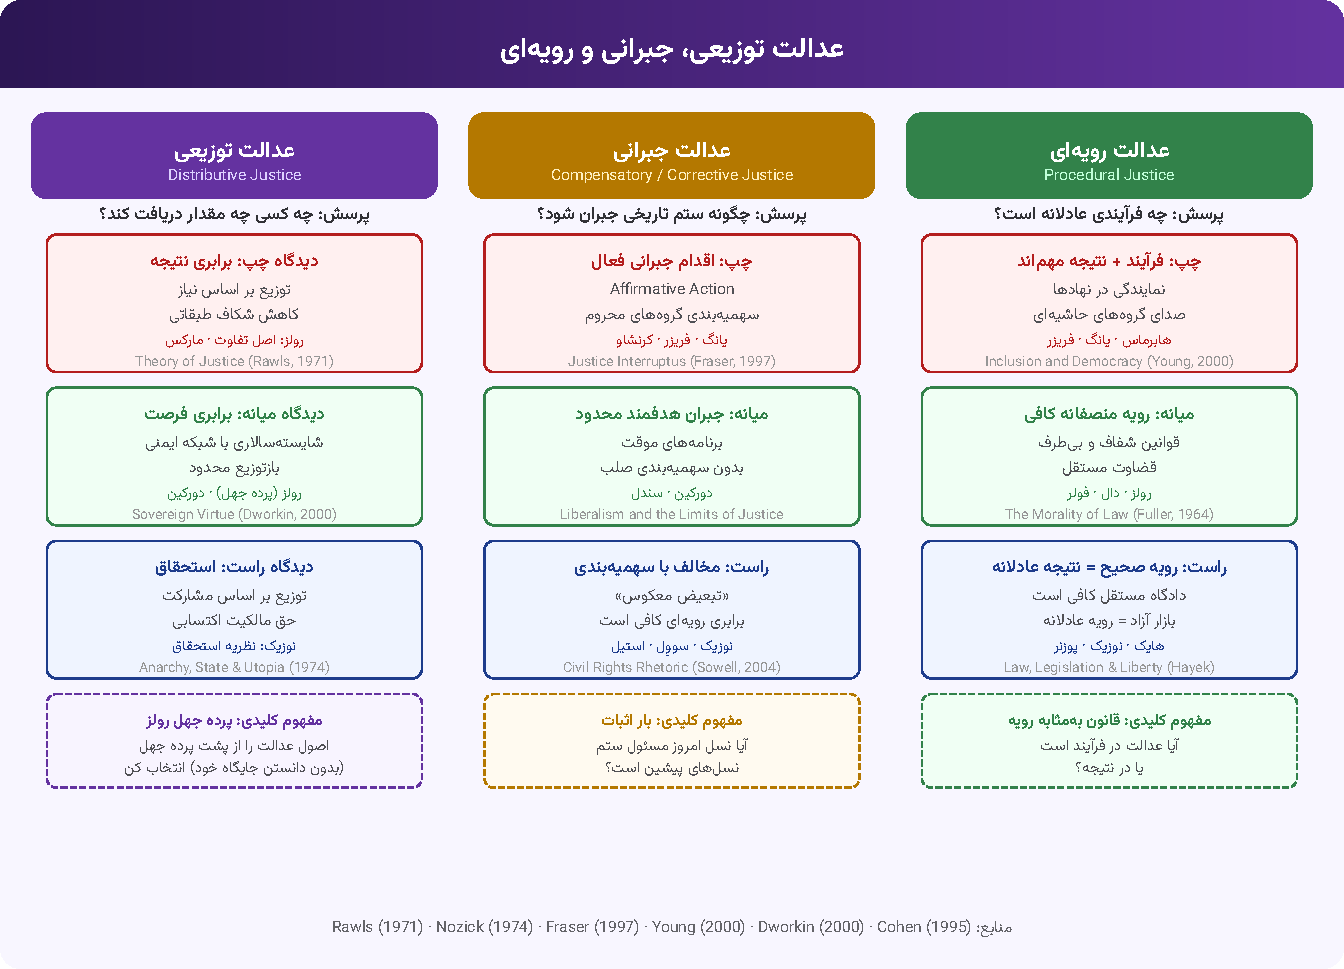
\includegraphics[width=\linewidth]{figures/infographic-justice.pdf}
  \caption{سه گونهٔ عدالت: توزیعی، جبرانی و رویه‌ای}
  \label{fig:justice}
\end{figure}

\begin{defbox}[پرده جهل رولز]
\begin{center}
\begin{tikzpicture}[every node/.style={font=\small}]
  \fill[DarkGray!80, rounded corners=6pt]
       (0,0) rectangle (12,3.8);
  \fill[DarkGray!40, rounded corners=4pt]
       (0.2,0.2) rectangle (5.8,3.6);
  \fill[DarkGray!40, rounded corners=4pt]
       (6.2,0.2) rectangle (11.8,3.6);
  \node[font=\bfseries\large, text=white] at (6,1.9)
       {\rl{پرده جهل}};
  \node[text=white!80, align=center, font=\footnotesize] at (3,2.8)
       {\rl{نمی‌دانی:}};
  \node[text=white!70, align=center, font=\footnotesize] at (3,2.2)
       {\rl{• ثروت خانواده}};
  \node[text=white!70, align=center, font=\footnotesize] at (3,1.7)
       {\rl{• استعداد فطری}};
  \node[text=white!70, align=center, font=\footnotesize] at (3,1.2)
       {\rl{• نژاد و جنسیت}};
  \node[text=white!70, align=center, font=\footnotesize] at (3,0.7)
       {\rl{• جایگاه اجتماعی}};
  \node[text=white, align=center, font=\footnotesize] at (9,2.8)
       {\rl{چه اصولی انتخاب می‌کنی؟}};
  \node[text=GoldLight, align=center, font=\footnotesize] at (9,2.2)
       {\rl{• آزادی برابر برای همه}};
  \node[text=GoldLight, align=center, font=\footnotesize] at (9,1.7)
       {\rl{• برابری فرصت عادلانه}};
  \node[text=GoldLight, align=center, font=\footnotesize] at (9,1.2)
       {\rl{• اصل تفاوت}};
  \node[text=GoldLight!80, align=center, font=\footnotesize] at (9,0.7)
       {\en{Rawls, 1971}};
\end{tikzpicture}
\end{center}
\mediumspace
\person{جان رولز} در \book{نظریهٔ عدالت} (۱۹۷۱) استدلال کرد
که اصول عادلانه آن‌هایی‌اند که انسان‌ها پشت «پردهٔ جهل» انتخاب می‌کنند.
\end{defbox}

\ornamentalrule

% ─────────────────────────────────────────────────────────────────
\section*{۸. مسئولیت فردی در برابر اجتماعی}
% ─────────────────────────────────────────────────────────────────

\begin{figure}[H]
  \centering
  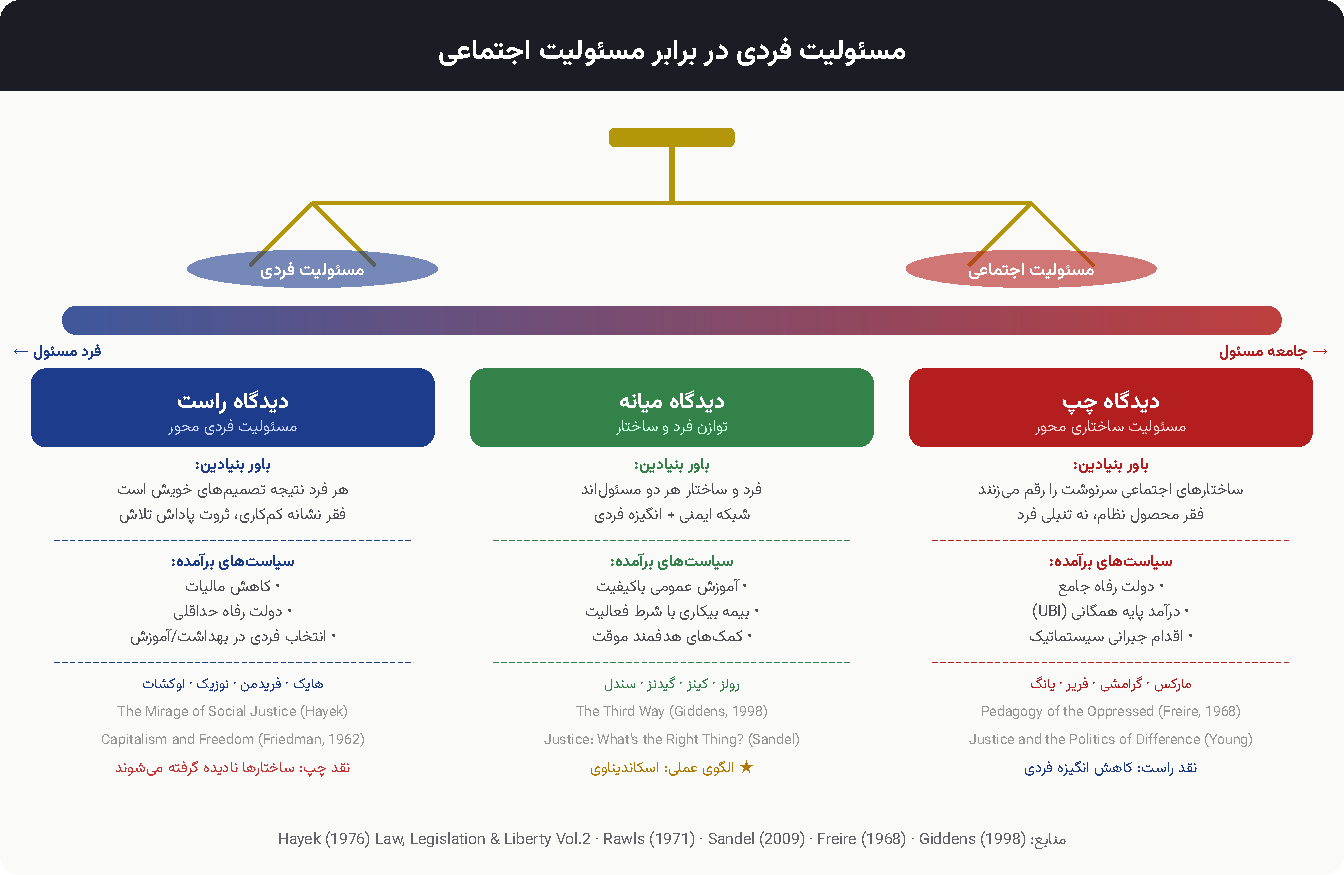
\includegraphics[width=\linewidth]{figures/infographic-responsibility.pdf}
  \caption{تقابل مسئولیت فردی و اجتماعی}
  \label{fig:responsibility}
\end{figure}

\ornamentalrule

% ─────────────────────────────────────────────────────────────────
\section*{۹. تقابل‌های اقتصادی}
% ─────────────────────────────────────────────────────────────────

\begin{figure}[H]
  \centering
  
\includegraphics[width=\linewidth]{figures/infographic-economy.pdf}
  \caption{مقایسهٔ رویکردهای اقتصادی در شش حوزه}
  \label{fig:economy}
\end{figure}

\begin{historybox}[پیکتی و بازگشت نابرابری]
\person{توما پیکتی} در \book{سرمایه در قرن بیست‌ویکم} (۲۰۱۳)
با داده‌های سیصدساله نشان داد:
\[
  r > g \implies \text{تمرکز ثروت افزایش می‌یابد}
$$
راه‌حل: مالیات تصاعدی جهانی بر ثروت.\\[4pt]
{\small\en{Piketty (2013),
\textit{Capital in the Twenty-First Century}, Harvard UP.}}
\end{historybox}

\ornamentalrule

% ─────────────────────────────────────────────────────────────────
\section*{۱۰. جدول جامع تقابل‌ها}
% ─────────────────────────────────────────────────────────────────

% FIXED: longtable با ستون‌های کوچک‌تر برای جلوگیری از overfull hbox
\begin{longtable}{
    >{\columncolor{DarkGray!8}\raggedleft\arraybackslash}p{2.8cm}
    >{\raggedright\arraybackslash}p{3.4cm}
    >{\raggedright\arraybackslash}p{3.4cm}
    >{\raggedright\arraybackslash}p{2.8cm}
    >{\raggedright\arraybackslash}p{2.4cm}
  }

\rowcolor{DarkGray!25}
\textbf{حوزه} &
\textbf{\textcolor{LeftRed}{چپ}} &
\textbf{\textcolor{CenterGreen}{میانه}} &
\textbf{\textcolor{RightBlue}{راست}} &
\textbf{منبع}
\\\hline
\endfirsthead

\rowcolor{DarkGray!25}
\textbf{حوزه} &
\textbf{\textcolor{LeftRed}{چپ}} &
\textbf{\textcolor{CenterGreen}{میانه}} &
\textbf{\textcolor{RightBlue}{راست}} &
\textbf{منبع}
\\\hline
\endhead

\hline
\endlastfoot

% اقتصادی
\rowcolor{RightBlue!6}
\multicolumn{5}{r}{
  \textbf{\textcolor{RightBlue}{\rl{▸ اقتصادی}}}}
\\\hline

مالکیت &
مالکیت اجتماعی &
اقتصاد مختلط &
مالکیت خصوصی &
\en{\footnotesize Nozick (1974)}
\\\hline

مالیات &
تصاعدی شدید &
تصاعدی معتدل &
مسطح یا حداقل &
\en{\footnotesize Piketty (2013)}
\\\hline

دستمزد &
حداقل زیستی بالا &
حداقل ملی &
بازار تعیین کند &
\en{\footnotesize Stiglitz (2012)}
\\\hline

تجارت &
حمایت داخلی &
تجارت آزاد + استانداردها &
آزادسازی کامل &
\en{\footnotesize Ricardo (1817)}
\\\hline

نابرابری &
تهدید دموکراسی &
معتدل قابل قبول &
انگیزه‌بخش &
\en{\footnotesize Rawls (1971)}
\\\hline

% سیاسی
\rowcolor{LeftRed!6}
\multicolumn{5}{r}{
  \textbf{\textcolor{LeftRed}{\rl{▸ سیاسی}}}}
\\\hline

دموکراسی &
مشارکتی &
لیبرال نمایندگی &
قانون اساسی محدود &
\en{\footnotesize Habermas (1996)}
\\\hline

نقش دولت &
هدایت‌گر &
تسهیل‌گر &
حداقلی &
\en{\footnotesize Hayek (1944)}
\\\hline

آزادی &
آزادی مثبت &
هر دو &
آزادی منفی &
\en{\footnotesize Berlin (1969)}
\\\hline

نظم سیاسی &
تغییر بنیادین &
اصلاح تدریجی &
حفظ سنت‌ها &
\en{\footnotesize Burke (1790)}
\\\hline

ملت‌گرایی &
انترناسیونالیسم &
همکاری + حاکمیت &
ناسیونالیسم &
\en{\footnotesize Walzer (1983)}
\\\hline

% اجتماعی
\rowcolor{CenterGreen!6}
\multicolumn{5}{r}{
  \textbf{\textcolor{CenterGreen}{\rl{▸ اجتماعی}}}}
\\\hline

آموزش &
عمومی رایگان &
عمومی باکیفیت &
رقابتی &
\en{\footnotesize Dewey (1916)}
\\\hline

بهداشت &
عمومی جهانی &
بیمه اجباری &
بازار رقابتی &
\en{\footnotesize Beveridge (1942)}
\\\hline

محیط زیست &
مقررات سخت &
مالیات کربن &
نوآوری بازار &
\en{\footnotesize Pigou (1920)}
\\\hline

جرم &
علل اجتماعی + اصلاح &
توانبخشی + بازدارندگی &
مجازات + مسئولیت فردی &
\en{\footnotesize Foucault (1975)}
\\\hline

مهاجرت &
مرزهای باز &
تنظیم‌شده &
کنترل سخت &
\en{\footnotesize Carens (1987)}
\\\hline

% عدالت
\rowcolor{GoldAccent!10}
\multicolumn{5}{r}{
  \textbf{\textcolor{GoldDark}{\rl{▸ عدالت}}}}
\\\hline

عدالت توزیعی &
برابری نتیجه &
برابری فرصت &
استحقاق &
\en{\footnotesize Rawls/Nozick}
\\\hline

عدالت جبرانی &
اقدام مثبت فعال &
جبران هدفمند &
مخالف سهمیه‌بندی &
\en{\footnotesize Fraser (1997)}
\\\hline

مسئولیت &
ساختار اجتماعی &
فرد + ساختار &
مسئولیت فردی &
\en{\footnotesize Sandel (2009)}
\\\hline

\caption{جدول جامع تقابل‌های موضوعی در ۱۸ حوزه}
\label{tab:comprehensive}
\end{longtable}

\vspace{6pt}

\begin{questionbox}
\begin{enumerate}[leftmargin=*, itemsep=8pt]
  \item اگر «پشت پردهٔ جهل» رولز قرار داشتید،
        کدام نظام توزیع ثروت را انتخاب می‌کردید و چرا؟

  \item آیا دموکراسی مشارکتی چپ و دموکراسی قانون اساسی راست
        می‌توانند با یکدیگر ترکیب شوند؟

  \item پیکتی نشان داد $r > g$؛ آیا این به معنای
        ناپایداری ذاتی سرمایه‌داری است؟

  \item مرز میان «آزادی منفی» و «آزادی مثبت» کجاست؟

  \item استروم نشان داد جوامع بدون دولت و بازار می‌توانند
        منابع مشترک را مدیریت کنند.
        این یافته چه چالشی برای هر دو طیف ایجاد می‌کند؟
\end{enumerate}
\end{questionbox}